\documentclass[11pt]{report}
\clubpenalty=10000
\widowpenalty=10000
%\usepackage[]{graphicx}
\usepackage[draft]{graphicx}
% It is handy to define new commands for text that occurs frequently (see Discussion)
\newcommand{\MT}{^{\mathrm{MT}}}
\newcommand{\ga}{\gtrsim}
\newcommand{\Lpot}{(L+1)^2}
\newcommand{\WS}{^{\mathrm{WS}}}
\newcommand{\fracd}[2]{\frac{\displaystyle{#1}}{\displaystyle{#2}}} 

%--Format the section headers

%\usepackage{nameref}
\usepackage{amsmath}
\usepackage{amsfonts}
\usepackage{amssymb}
\usepackage{wasysym}
\usepackage{graphicx}
\usepackage{pslatex}
\usepackage{lscape}
\usepackage[T1]{fontenc}
\usepackage[latin1]{inputenc}
\usepackage{longtable}
 \setlength{\LTcapwidth}{5.5 in}
\usepackage{chapterbib}
\usepackage{fancyhdr} % for better header layout
\usepackage{eucal}
\usepackage[english]{babel}
\usepackage[usenames, dvipsnames]{color}
\usepackage[perpage]{footmisc}
\usepackage[round, sort, numbers, authoryear]{natbib}
%\usepackage{multicol} % for pages with multiple text columns, e.g. References
\setlength{\columnsep}{20pt} % space between columns; default 10pt quite narrow
\usepackage[nottoc]{tocbibind} % correct page numbers for bib in TOC, nottoc suppresses an entry for TOC itself
\usepackage{geometry}
\usepackage{setspace}
\usepackage{url}
\usepackage{lastpage}

% FJS Changed this... I didn't like the numbering or the
% indentation... so I introduced a fake chapter Main Text. 
\setcounter{secnumdepth}{0}
\setcounter{tocdepth}{5}

%--set the page formatting--
\geometry{hmargin={1.6in,1.1in},vmargin={1.5in,1.2in}}
\doublespacing

\begin{document}
%--front matter needs roman pagination--
\pagenumbering{roman}

%--Title Page--
\thispagestyle{empty}
  \begin{center}
    \textsc{\LARGE Using Princeton Precipitation climatology to predict future precipitation events} %Fill in your information
  \end{center}
  \vspace{.6in}
  \begin{center}
      Tyrone Zhang
  \end{center}
  \vspace{.6in}
  \begin{center}
    \textsc{A Senior Thesis \\ %Fill in your information
    Presented to the Faculty \\
    of Princeton University \\
    in Candidacy for the Degree \\
    of Bachelor of Arts}
  \end{center}
  \vspace{.3in}
  \begin{center}
    \textsc{Recommended for Acceptance \\
    by the \\Department of  Geosciences \\}
    Adviser: Frederik J.~Simons
  \end{center}
  \vspace{.3in}
  \begin{center}
  \today
  \end{center}
  
  \clearpage


%--Copyright Page--
\thispagestyle{empty}
\vspace*{3in}
\begin{center}
\emph{This paper represents my own work in accordance with University regulations,} \\
Tyrone Zhang %%Sign here
\end{center}
\clearpage

%--Abstract--  
\addcontentsline{toc}{chapter}{Abstract}
\begin{center}
\Large \textbf{Abstract}
\end{center}
 
% Senior thesis or Junior Project Abstract -----------------------------------------------------

%Delete the text below and write your abstract
Princeton's climate is one that has four seasons and a high temperature variation through the year. The precipitation in Princeton is spread out throughout the year. Precipitation events are often characterized by an exponential distribution of both the duration and the total precipitation per event. The shortest precipitation events and the smallest precipitation totals are the most frequent, while the longer the precipitation event, the less likely it is to occur at any given point.  By analyzing the precipitation that is measured from Professor Simons' Vaisala weather station on the top of Guyot Hall from 2017 to present day, I can first summarize the data that is being characterized, then start using this climatology to start predicting precipitation events based on other variables that are observed in the weather station. 

 \clearpage

%--Acknowledgements--  
\addcontentsline{toc}{chapter}{Acknowledgements}
\begin{center}
\Large \textbf{Acknowledgements}
\end{center}

% Senior thesis or Junior Project Acknowledgements  -----------------------------------------------------

%Delete the text below and write your acknowledgements
I would like to acknowledge my senior thesis advisor Frederik J. Simons for giving me constant feedback on my work as well as providing me with the data that he is collecting on top of Guyot Hall. His patience and guidance through this tough year was welcomed for sure. I also thank Professor Alan Rubin for being my second reader. 

I also like to acknowledge my family, who has been very supportive and understanding in my time in Princeton, especially during this past year. 

My Princeton friends who were also in the thesis grind who were also struggling over the past year. Our common struggle helped us bond in these rather tough times. 

Finally all those in the Geoscience department, especially my fellow seniors in which we tried to make the best out of a weird situation for our seniors. 
\clearpage

%--Table of Contents--  
\thispagestyle{empty}
\tableofcontents
\clearpage

\listoffigures 
\listoftables
\clearpage

%--Set up fancy header-- 
\fancyhead{}
\fancyfoot{}
\pagestyle{fancyplain}
\rhead{\fancyplain{\thepage}{\noindent \textsc{\rightmark} \hfill \thepage~of~\pageref{LastPage}}}
\rfoot{\hrule \today \hfill Tyrone Zhang}
\pagenumbering{arabic}

%--Reset the page numbers and set them to arabic-- 
{\newpage\renewcommand{\thepage}{\arabic{page}}\setcounter{page}{1}}

%--Have sections but use chapter counters
\addcontentsline{toc}{chapter}{Main Text}

\section{Introduction}\label{sec:introduction}

The climatology of Princeton is one that belongs to the mid-latitudes, which
is characterized by having four seasons that results in a large variation in
temperature throughout a year. In terms of the average calculated between
1981 and 2010, Princeton gets an average of 1227~mm of precipitation
annually, and the precipitation distribution throughout the year is fairly
even, with less precipitation in the winter~\cite[]{PRISM}.  According to
the Koppen-Geiger Climate Classification, Princeton, NJ lies in the
classification Cfa, which denotes a temperate climate, with no dry season,
and hot summers defined as reaching~22$^\circ$C or higher
\cite[]{Peel2008}. Princeton having no dry season means that precipitation
is well spread out throughout the year.

% %\documentclass[12pt]{article}
%\usepackage[margin=1in]{geometry} 
%\usepackage{amsmath,amsthm,amssymb,amsfonts}
%\usepackage{graphicx}
%\usepackage{float} 
%\newcommand{\N}{\mathbb{N}}
%\newcommand{\Z}{\mathbb{Z}}
%\newenvironment{problem}[2][Problem]{\begin{trivlist}
%		\item[\hskip \labelsep {\bfseries #1}\hskip \labelsep {\bfseries #2.}]}{\end{trivlist}}
%\begin{document}

\begin{figure}[h]
\centering
\includegraphics0.75\textwidth{../Figures/intensity_hist_5min.png}
\caption{\label{abc}Distribution of intensity of precipitation events in 2019,
defined as the total precipitation divided by the duration. This
distribution was derived from the distribution of duration of
precipitation with a minimum duration of 5 minutes. The distribution
decreases logarithmically from 0.01 mm/minute to 0.5 mm/minute.} 
\end{figure}
\vfill
\begin{figure}[h]
\centering
\includegraphics0.75\textwidth{../Figures/intensity_hist_1min.png}
\caption{\label{abcd}Distribution of intensity of precipitation events in 2019,
defined as the total precipitation divided by the duration. This
distribution was derived from the distribution of duration of
precipitation with a minimum duration of 1 minute. The distribution
decreases logarithmically from 0.01 mm/minute to 0.5 mm/minute.} 
\end{figure}
\vfill
\begin{figure}[h]
\centering\includegraphics0.75\textwidth{../Figures/precip_hist_5min.png} 
\caption{\label{abce}Distribution
of duration of precipitation events in 2019. 5 minutes was the minimum
duration needed to define a precipitation event. The distribution is
decreasing logarithmically from the highest values in the 5 minute
precipitation events and the lowest values approaching 100 minutes.}
\end{figure}
\begin{figure}[h]
\centering
\includegraphics0.75\textwidth{../Figures/precip_hist_1min.png}
\caption{\label{abcf}A histogram that shows the duration of precipitation
event. Note that in this histogram that the 1 minute was the minimum
duration needed to define a precipitation event. As expected, the
distribution is that we have most precipitation events be close to the
minimum duration and that less precipitation events are particularly
long. } 
\end{figure}
\begin{figure}[h]
\centering \includegraphics0.75\textwidth{../Figures/nonprecip_hist_5min.png} 
\caption{\label{abcg}This is a histogram for the duration of a
non-precipitation event, which is to say the gap between two
precipitation events. It also follows the pattern of having lots of
the non-precipitation events be close to the minimum non-precipitation
event of 5 minutes. It does look like that there are more
non-precipitation events that lasts longer than say 40 minutes
compared to the precipitation events. }
\end{figure}
\begin{figure}[h]
\centering
\includegraphics0.75\textwidth{../Figures/nonprecip_hist_1min.png}
\caption{\label{abch}This is a histogram for the duration of a non-precipitation
event, which is to say the gap between two precipitation events. Most
events do seem to lie close to the minimum duration of 1 minute.} 
\end{figure}
\begin{figure}[h]
\centering 
\includegraphics0.75\textwidth{../Figures/nonprecip1mm_season_19.png} 
\caption{\label{abci}Distribution of the duration of non-precipitation
events separated by seasons. The distribution within each season does
indeed decrease exponentially as we go from 1 minute duration to about
40 minute duration, with the extreme 98th to 100th percentile
excluded.}
\end{figure}
\begin{figure}[h]
\centering
\includegraphics0.75\textwidth{../Figures/precip1mm_season_19.png}
\caption{\label{abcj}Distribution of the duration of precipitation events
separated by seasons. The distribution for each season does decrease
exponentially from 1 minute to 40 minute durations. It does seem like
the more precipitation events are closer to the minimum precipitation
duration compared to the non-precipitation events.} 
\end{figure}
\begin{figure}[h]
\centering \includegraphics0.75\textwidth{../Figures/inten1mm_season_19.png} 
\caption{\label{abck}Distribution of intensity of precipitation events
separated by seasons. The distribution decrease for each season from
0.01 mm/minute to 0.27 mm/day.}
\end{figure}
\begin{figure}[h]
\centering
\includegraphics0.75\textwidth{../Figures/inten1mm_season_19_log.png}
\caption{\label{abcl}Shows the previous figure in terms of log scale for both x
and y axis. It shows that winter does not have very intense
precipitation events and that despite Summer and Winter having similar
amounts of precipitation, (232 mm for Summer to 240 mm for Winter),
summer seems to have more intense precipitation events.}
\end{figure}
%\end{document}


The weather station on the top of Guyot Hall is Vaisala weather transmitter
WXT530 series. It measures six weather parameters of air pressure,
temperature, humidity, rainfall, wind speed, and wind direction. The
rainfall is measured using an acoustic Vaisala RAINCAP Sensor, which helps
avoid the complications of flooding, wetting, and evaporation losses
\cite[]{Vaisala}. In Figure~\ref{daily}, the fluctuations of 
meteorological variables occurs throughout the day.   

Air temperature is the temperature that the thermometer measures when
exposed to the air, while sheltered from direct solar radiation.
Atmospheric pressure is the pressure exerted by the atmosphere due to
gravitational attraction on the air column above a point in question
\cite[]{AMS}. Relative humidity is the ratio of vapor pressure to saturation
vapor pressure with respect to water \cite[]{AMS}.  This means that two air
parcels can hold the same amount of water vapor, but if one air parcel is
warmer than the other parcel, the higher temperature air parcel has a lower
relative humidity than the lower temperature air parcel because warmer air
has a higher saturation vapor pressure for water.  Precipitation
accumulation is the amount of water substance that has fallen at a given
point over a specified period of time \cite[]{AMS}.

%At the same time, relative humidity becomes important especially during
%warmer temperatures, as increases in relative humidity can mean the
%apparent temperature felt by humans will increase. This is the heat index,
%in which

\begin{figure}[thb]
\centering 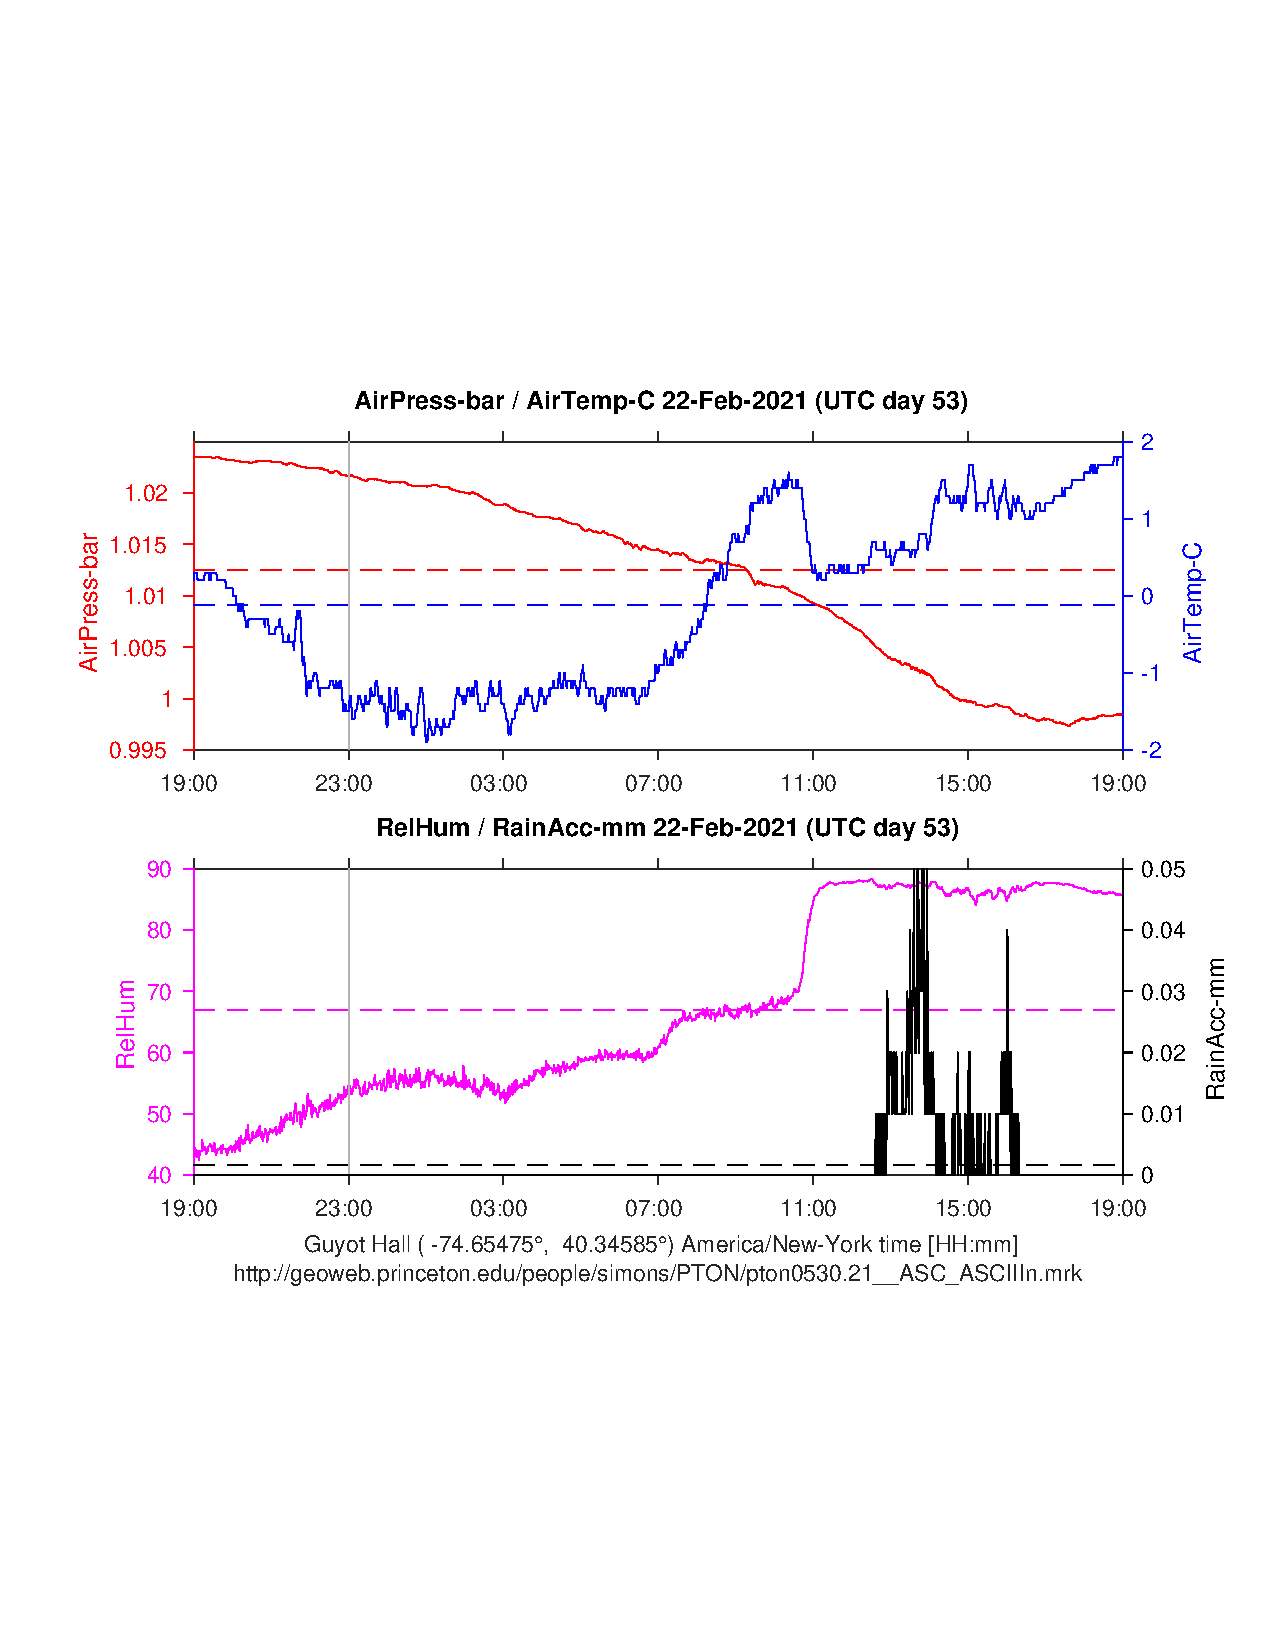
\includegraphics[trim = 0.5cm 5.0cm 0.5cm 6.0cm,clip,width=1.0\textwidth]
{Figures/guyotweather_ywt_feb_22_2021.pdf}
\caption[Weather Station Data]{\label{daily}A daily plot of the
  meteorological variables that the Vaisala station measures on top
  of Guyot Hall.}
\end{figure}

% FJS BASIC CLIMATOLOGY FIGURES TEMPERATURE, PRECIPITATION, RELHUM

From the data analyzed, the following is the climatology of Princeton from
2017 to 2021. Looking at Figure~\ref{Clim1}, temperature
and precipitation that varies throughout the year. Temperatures start
increasing before peaking in July, before decreasing until January. This is
consistent with the fact that Princeton has four seasons, which shows cold
winters, warm summers, and mild spring and fall. At the same time, there is
more precipitation in the spring and summer compared to the relative lack of
precipitation in the fall and winter.

The month with the lowest average precipitation is January, at an average
monthly precipitation of 44~mm, whereas the month with the highest average
precipitation is July with 123~mm.

Figure~\ref{Temp_range}, shows that the ranges of temperature are not equal
throughout the months. For example, winter months of January and Feburary
have a big range that spans from about $20 ^\circ $C to $-10
^\circ$C. Meanwhile, summer months such as July and August, whose
range of temperatures is smaller, from about $30 ^\circ $C to about $15
^\circ $C.

The relative humidity for Princeton is higher in the months of
August to October, whereas the lowest relative humidity seems to be in the
months of March and April.  With Figure~\ref{RH_range}, all
the months have similar upper extremes of about 90\% for relative humidity,
which can indicate precipitation. At the same time, the range for relative
humidity is largest in the spring time, with March, April, and May seem to
have a range between 15\% to 90\% for relative humidity, with caution that
this is just data from 3 years.

For atmospheric pressure, the lowest monthly air pressure are found in the
months of April and June, while the highest monthly air pressure are found
in the month of Feburary. Though the values for the mean atmospheric
pressure are all pretty close to each other ranging from about 1.00~bar to
1.01~bar. The more interesting aspects of atmospheric pressure comes from
the range of atmospheric pressure, where the months of May to September all
seem to have a small range that vary between 0.995~bar to about
1.02~bar. Meanwhile months like October, which have a larger range
of atmospheric pressure, which ranges from 0.97~bar to 1.03~bar. Clearly
these low atmospheric pressure must come from an intense low pressure that
passed near Princeton. It turns out that for the month of October from
2017-2020, the values between 0.97~bar to 0.985~bar represent
the 0 to 1st percentile of all atmospheric pressures for the month of
October, so they are relatively low pressures. Other months such as November
to February have relatively large ranges for atmospheric pressure as well.
\clearpage
\begin{figure}[b]
	\centering
	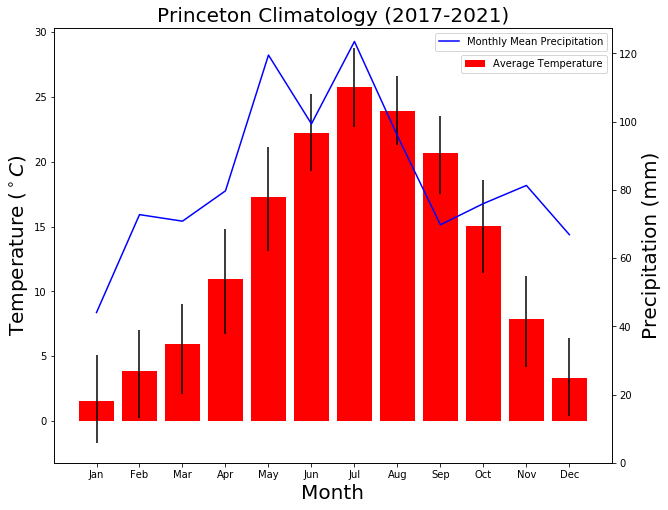
\includegraphics[width=0.675\textwidth]{Figures/Climate1.png}
	\caption[Climatology of temperature and precipitation of Princeton
          (2017--2021)]{\label{Clim1} Climatology shown for Princeton from
          August 2017 to January 2021. The black interval lines show the
          25--75th interpercentile range for temperature of the month.}
\end{figure}

\begin{figure}[b]
	\centering
	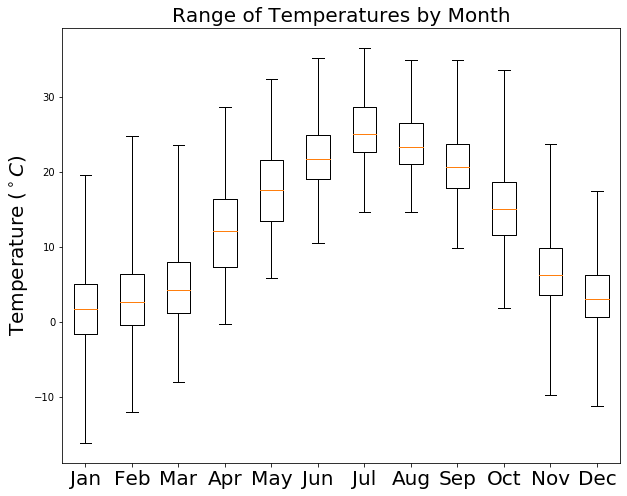
\includegraphics[width=0.675\textwidth]{Figures/Temp_range.png}
	\caption[Temperature range for Princeton
          (2017--2021)]{\label{Temp_range} Shows the interpercentile ranges
          as a bar and the mean temperatures as a line graph. The whiskers
          go out to the 0th percentile and 100th percentile, respectively.}
\end{figure}
\clearpage

%FJS In Section~{\textit{\nameref{sec:dcp}} I show this and that. 
% Will add 25-75th percentile range, since I think that would make sense. 
 % Again will add 25-75th percentile ranges too, since it would also make sense! 
\clearpage

\begin{figure}[t]
	\centering
	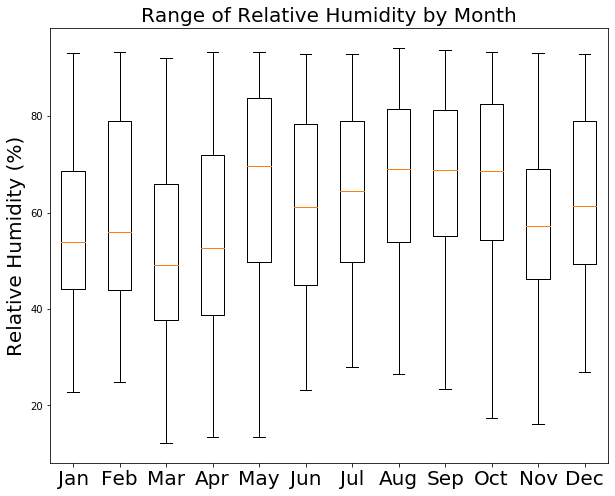
\includegraphics[width=0.65\textwidth]{Figures/RH_range.png}
	\caption[Range of Relative Humidity in Princeton
          (2017--2021)]{\label{RH_range} Range of relative humidity for
          Princeton with the mean relative humidity for the month indicated
          by the orange line.}
\end{figure}
\begin{figure}[b]
	\centering
	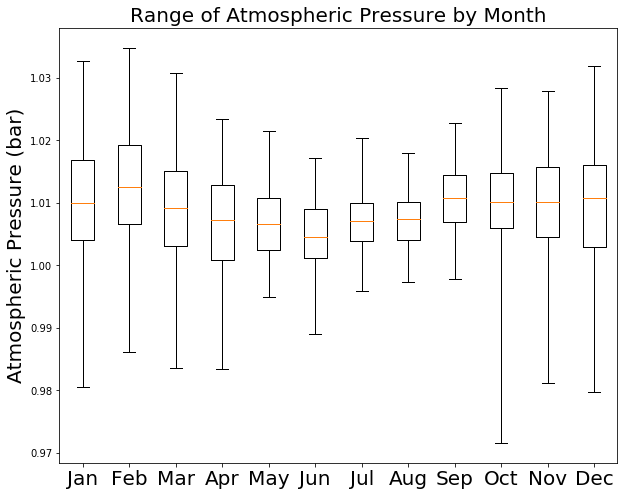
\includegraphics[width=0.65\textwidth]{Figures/AP_range.png}
	\caption[Range of Atmospheric Pressure in Princeton (2017--2021)
        ]{\label{AP_range} A graph similar to Figure~\ref{RH_range} looking
          at range of atmospheric pressure through out the months.}
\end{figure}
\clearpage
\section{Descriptive Climatology of Precipitation}\label{sec:dcp}

Despite the information given to us in looking the ranges of meteorological
variables like temperature, relative humidity, and atmospheric pressure,
precipitation events are no where to be seen.  I shall define the following
terms. The time series of \textbf{precipitation} as recorded by the
instrument is denoted $e_i$, where $i$ indexes the measurement intervals,
each 60~s long. I define a precipitation \textbf{event} $E_j^\tau $ as a
sequence of \textbf{duration} $d_j\ge \tau$ containing contiguous nonzero
precipitation measurements $e_i>0$, flanked left and right by zeros,
$e_i=0$, and where $\tau$ is in minutes \cite[]{Eagleson}.

Furthermore, I define a non-precipitation \textbf{event} $N_j^\tau$, as
having a contiguous set of zeros, $e_i=0$, whose combined duration exceeds
$\tau$, flanked left and right by non-zero values, $e_i=0$ \cite{Eagleson}.
% Basically we want the hand-drawn figure shown here!
One more term to define is \textbf{precipitation intensity}, which for a
precipitation event $E_j^\tau$ is the total amount of precipitation divided
by its duration, i.e.,
\begin{equation}
  I_j^\tau = \fracd{\sum_i e_i }{d_j} ,
  \quad
  \mbox{for}\,\,\,\, i\,\,\,\, \mbox{belonging to the event}\,\,\,\, E_j^\tau
  .
\end{equation}

For further analysis, I am breaking down the year into seasons, as different
seasons may have different characteristics with regards to precipitation. I
will define the seasons as follows: Winter will be December, January, and
February. `Winter' of a certain year contains December of the previous
year. Spring will be March, April, and May. Summer is June, July, and
August. Fall is September, October, November.

The following histograms show the distribution of precipitation event
duration in terms of minutes and shows the different duration distributions
per season. For precipitation and non-precipitation events, $\tau = 1$~min,
which means all precipitation and non-precipitation events that are 1 minute
or longer in duration accounted for. 

\clearpage
\begin{figure}[t]
  \centering
  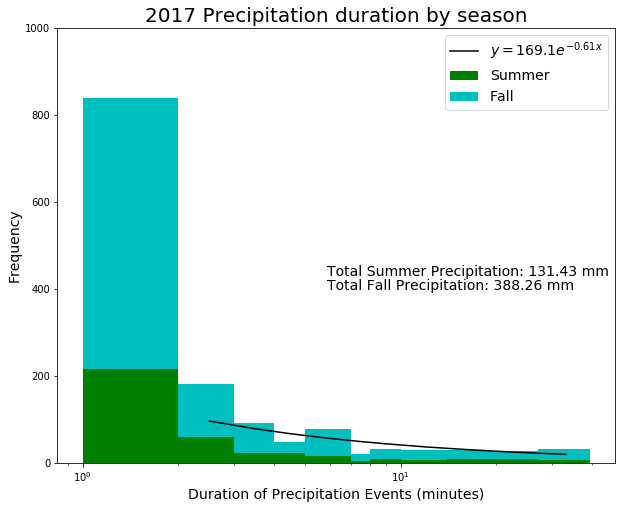
\includegraphics[width=0.675\textwidth]{Figures/precip_2017.png}
  \caption[Precipitation histogram for 2017 broken down by
    season]{\label{p2017} Distribution of precipitation duration in 2017,
    with a breakdown by seasons. The minimum duration is $\tau = 1$~min.
    Note that data collection began on 16 July 2017. Which means only
    part of summer and all of the fall data are represented.  }
\end{figure}
\begin{figure}[b]
  \centering
  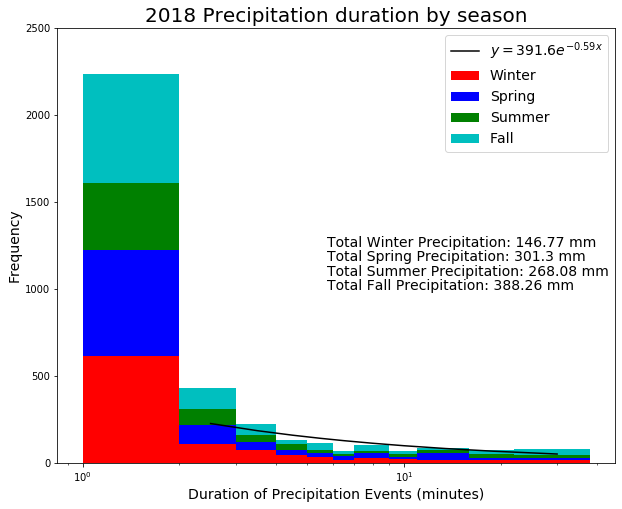
\includegraphics[width=0.675\textwidth]{Figures/precip_2018.png}
  \caption[Precipitation histogram for 2018 broken down by
    season]{\label{p2018} Distribution of precipitation duration in 2018,
    with a breakdown by seasons. 2018 is the first full year of data
    collections. The minimum duration is $\tau = 1$~min.}
\end{figure}

\clearpage
\begin{figure}[t]
  \centering
  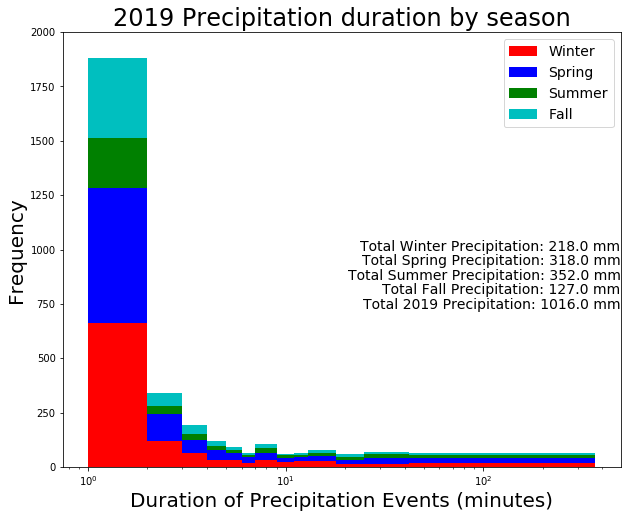
\includegraphics[width=0.675\textwidth]{Figures/precip_2019.png}
  \caption[Precipitation histogram for 2019 broken down by season]
          {\label{p2019}Distribution of precipitation duration in 2019, with
            a breakdown by seasons. The minimum duration is $\tau = 1$~min.
            %The minimum duration, $\tau=1$~min, and the maximum duration over the data
            %set is 368 min, but the horizontal axis was limited to the 98th percentile
            %of the durations, 42~min, for clarity. Superposed is a least-squares fit of
            %a line in log-log space of duration versus frequency for the entire year,
            %excluding the 1--2~min bin, quoted as the equivalent exponential in this
            %space.  
          }
\end{figure}

\begin{figure}[b]
  \centering
  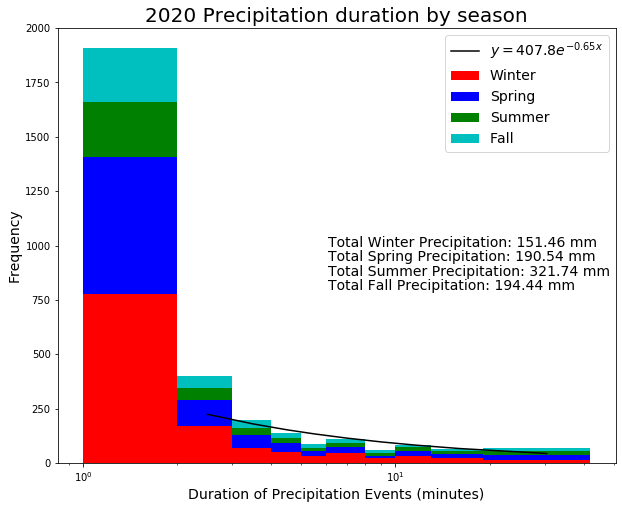
\includegraphics[width=0.675\textwidth]{Figures/precip_2020.png}
  \caption[Precipitation histogram for 2020 broken down by
    season]{\label{p2020}Distribution of precipitation duration in 2020,
    with a breakdown by seasons. The minimum duration is $\tau=1$~min. The
    layout is as in Figure~\ref{p2019}.}
\end{figure}

\clearpage

\begin{figure}[t]
	\centering
	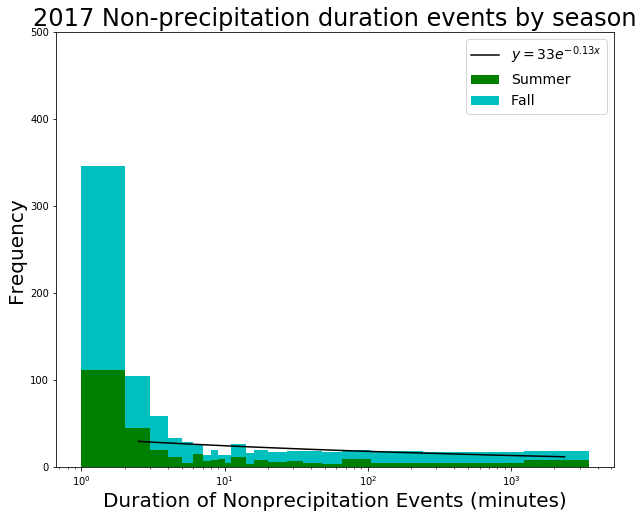
\includegraphics[width=0.675\textwidth]{Figures/nonprecip_2017.png}
	\caption[Histogram of non-precipitation events for 2017 broken down
          by season]{\label{np2017} Distribution of non-precipitation event
          duration in 2017, with a breakdown by seasons. The minimum
          duration is $\tau = 1$~min. Note that data collection began on 16
          July 2017, which means that summer is only partially complete.}
\end{figure}
\begin{figure}[b]
	\centering
	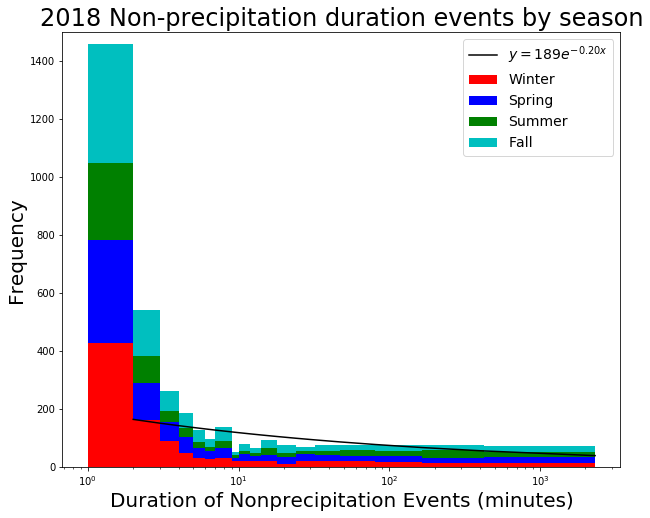
\includegraphics[width=0.675\textwidth]{Figures/nonprecip_2018.png}
	\caption[Histogram of non-precipitation events for 2018 broken down
          by season]{\label{np2018} Distribution of precipitation duration
          in 2018, with a breakdown by seasons. The minimum duration is
          $\tau=1$~min.}
\end{figure}

\clearpage
\begin{figure}[t]
	\centering
	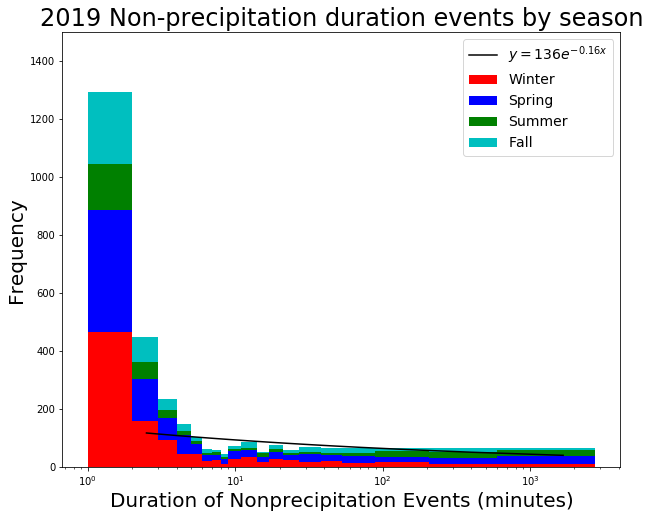
\includegraphics[width=0.675\textwidth]{Figures/nonprecip_2019.png}
	\caption[Histogram of non-precipitation events for 2019 broken
	down by season]{\label{np2019} Distribution of
		non-precipitation event duration in 2019, with a breakdown
		by seasons. The minimum duration is $\tau=1$~min. %, and the
		%maximum duration over the data set is 2613~min, but the
		%horizontal axis was limited to the 98th percentile of
		%2350~min, for clarity. Superposed is a least-squares fit of
		%a line in log-log space of duration versus frequency for the
		%entire year, excluding the 1--2~min bin, quoted as the
		%equivalent exponential in this space.
	}
\end{figure}

\begin{figure}[b]
	\centering
	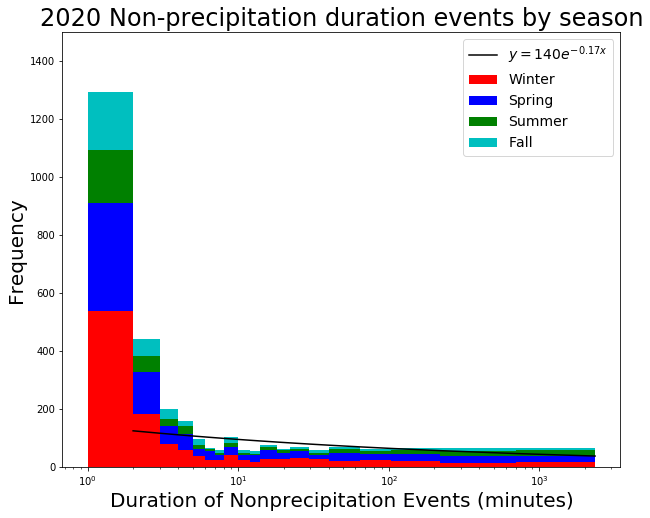
\includegraphics[width=0.675\textwidth]{Figures/nonprecip_2020.png}
	\caption[Histogram of non-precipitation events for 2020 broken down
          by season]{\label{np2020} Distribution of non precipitation event
          duration in 2020, with a breakdown by seasons. The minimum
          duration is $\tau=1$~min.}
\end{figure}


\clearpage
\begin{figure}[t]
  \centering
  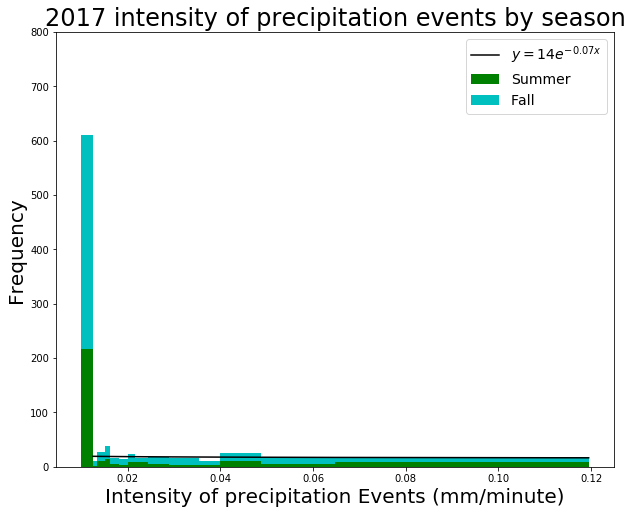
\includegraphics[width=0.675\textwidth]{Figures/inten2017.png}
  \caption[Intensity histogram for 2017 broken down by season]
          {\label{i2017}Distribution of precipitation intensity in 2017,
            with a breakdown by seasons. Note that data collection began on
            16 July 2017. The minimum intensity is $I=0.01$~mm/min}
\end{figure}
\begin{figure}[b]
  \centering
  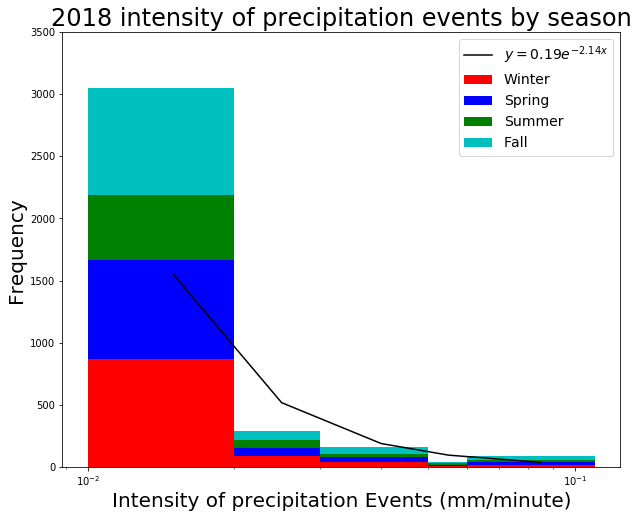
\includegraphics[width=0.675\textwidth]{Figures/inten2018.png}
  \caption[Intensity histogram for 2018 broken down by season]
          {\label{i2018}Distribution of precipitation intensity in 2018,
            with a breakdown by seasons. The minimum intensity is
            $I=0.01$~mm/min}
\end{figure}
\clearpage
\begin{figure}[t]
  \centering
  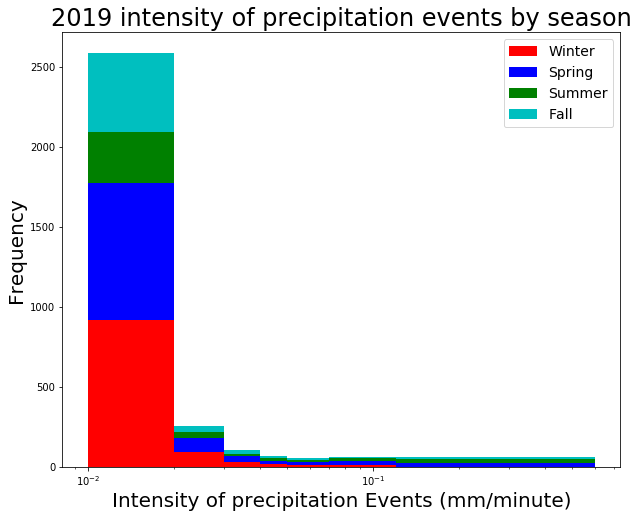
\includegraphics[width=0.675\textwidth]{Figures/inten2019.png}
  \caption[Intensity histogram for 2019 broken down by season]
          {\label{i2019}Distribution of precipitation intensity in 2019,
            with a breakdown by seasons. The minimum intensity is
            $I=0.01$~mm/min.  }
\end{figure}
\begin{figure}[b]
  \centering
  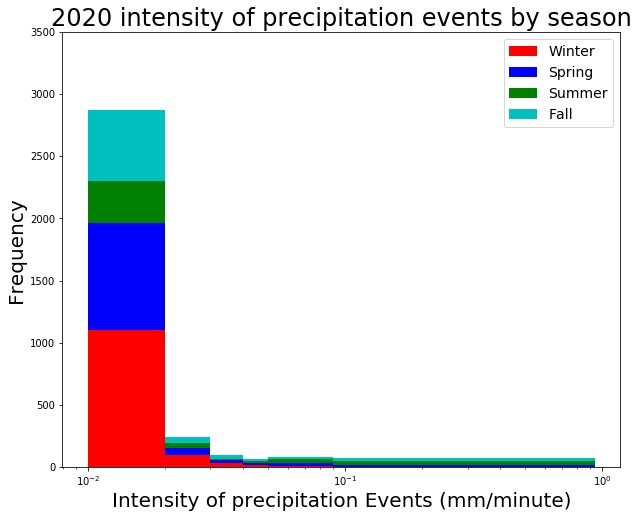
\includegraphics[width=0.675\textwidth]{Figures/inten2020.png}
  \caption[Intensity histogram for 2020 broken down by season]
          {\label{i2020} Distribution of precipitation intensity in 2020,
            with a breakdown by seasons. The minimum intensity is
            $I=0.01$~mm/min.}
\end{figure}
\clearpage

These histograms show that the smallest duration events for both
nonprecipitation and precipitation events are the most numerous as seen with
the largest bar in the bins that contain 1 minute to 2 minute durations. The
frequency of duration decreases as duration bins increase in value. At the
same time, there are differences between the precipitation and
non-precipitation events: the upper limit for duration of precipitation
events are about 300 to 400 minutes. However, the upper limit for duration
of non-precipitation events is about an order of magnitude greater at about
2000 minutes. Basically non-precipitation events can be as long as one or
two whole days, where as precipitation events can only last as long as 5-6
hours.

The intensity histogram shows an even stronger aggregation in the lowest
intensity bin of 1~mm/hour to 2~mm/hour. It is interesting because the small
intensity bin can include events that are long but less intense and short,
less intense precipitation events.

\section{Analysis of Precipitation}\label{sec:apc}

% FJS Here I do something. 

\subsection{Methods}\label{sec:methods}

With the climatology of precipitation characterized,the building predictive models for precipitation can be started. These models need a way to compare with each other as well as comparing the model results to the observed data. Such accuracy can be defined to check whether the model and the observed data match in terms existing precipitation at a given minute. The non-precipitation events should be ignored when looking at accuracy because by matching non-precipitation minutes in both the model and the observed data, the accuracy is over 90\%, which is not as useful. So, if the model and the
observed data do not match in terms whether there exists precipitation, this
contributes to the model being deemed less accurate. The accuracy will also measure the performance of the model, so the correct minutes to overall amount of minutes will be based on the model's total precipitation duration. 

%We can have a stricter
%definition of accuracy, in which we set up the precipitation condition, in
%addition to saying that the intensity must match too, otherwise we can not
%say the model and observed data match. This stricter definition of model
accuracy might be used when thinking about whether the intensity is being matched as well. Although this strict definition will not be used for this paper. 

\subsection{Results}\label{sec:apcr}

Figure~\ref{p2019} shows the distribution of durations of 3198 precipitation
events $E_j^1$, i.e. $E_j^\tau$ where $\tau=1$~min for the year 2019, broken
down by season. In order to make bins that contain non-zero values, I
created bins using duration percentiles. I used unique values obtained from
using a range of percentiles from 0 to 100, in 2 and 5 percent
intervals. For one analysis, I stopped at 98 \% believing this would be the
best approach in terms of fitting. At the same time, I also made sure to
analyze the data including the 100 percentile, to see how it differs when
including the extremes. Such purpose is also to realize that excluding such
extremes produced modelled precipitation that did not last long as well as
well as the gaps between precipitation events being too small.

I used an exponential fit to the frequency-duration histograms for all 1253
events $E_j^2$, i.e. $E_j^\tau$ where $\tau=2$~min. For all the other years,
as shown in Figures~\ref{p2020}, \ref{p2018} and~\ref{p2017}, I used a
similar procedure. Excluding the first interval shown, focusing on events of
duration greater than or equal to 2~min, I propose an exponential model for
the histogram, with the following equation:
\begin{equation}\label{expod}
  F = \beta \,e^{\alpha d},
\end{equation}
where $F$ is the frequency and $d$ the duration, and with $\beta$ the
unitless frequency coefficient and $\alpha$ is the exponential coefficient
(in units of min$^{-1}$). Table~\ref{firsttable} shows the
coefficients~$\beta$ and the exponential coefficients~$\alpha$ from looking
at the yearly frequency of precipitation duration.

I shall also propose the following equations which will also describe an
exponential model for the histogram regarding non-precipitation events,
which is described by the following equation:
\begin{equation}\label{expod_np}
	F_{np} = \gamma \,e^{\delta D},
\end{equation}
where $F_{np}$ is the frequency of non-precipitation events, $D$ being
duration, and $\gamma $ being the unitless frequency coefficient and
$\delta$ is the exponential coefficient. Table~\ref{thirdtable_98} shows the
coefficients~$\gamma$ and exponential coefficients~$\delta$ from looking at
yearly frequency of non-precipitation event durations.

A similar equation for precipitation intensity can be described by the
following equation:
\begin{equation}\label{expod_inten}
  F_{inten} = \epsilon \,e^{\zeta I},
\end{equation}
where $F_{inten}$ is the frequency of intensity of precipitation events, $I$
is the intensity of the precipitation events, $\epsilon$ is the unitless
frequency coefficient, and $\zeta$ is the exponential
coefficient. Table~\ref{fourthtable} shows the coefficients~$\epsilon$ and
the exponential coefficients~$\zeta$ from looking at yearly frequency of
intensity of precipitation events.

\clearpage
\begin{figure}[t]
\centering
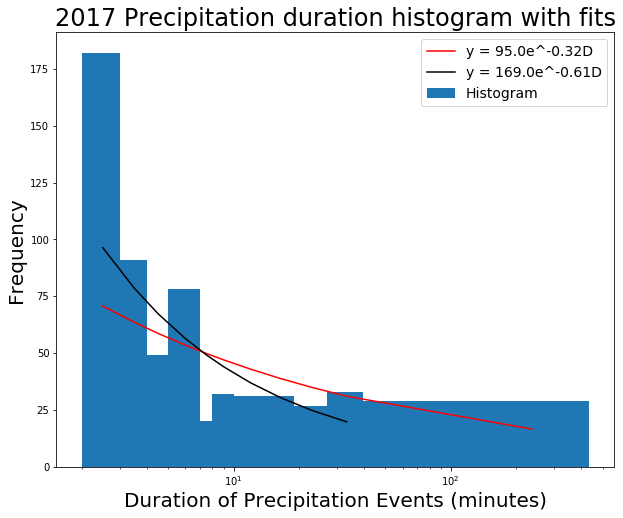
\includegraphics[width=0.625\textwidth]{Figures/precip17_new.png}
\caption[2017 precipitation duration exponentials with contrasting curve
  fitting] {\label{precip17_redone}Curve fitting of the precipitation
  histogram excluding 1 minute duration events for the incomplete 2017
  data. The red curve denotes the curve that fits to the 100th percentile,
  while the black curve fits the data to the 98th percentile. Has similar
  trends to the other years, though 2017 has incomplete data.}
\end{figure}

\begin{figure}[b]
\centering
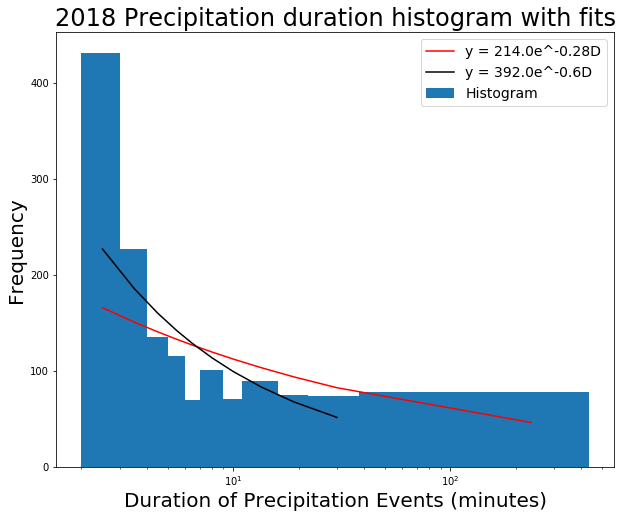
\includegraphics[width=0.625\textwidth]{Figures/precip18_new.png}
\caption[2018 precipitation duration exponentials with contrasting curve
  fitting] {\label{precip18_redone}Curve fitting of the precipitation
  histogram excluding 1 minute duration events for the entire 2018
  data. Format is the same as Figure~\ref{precip17_redone}, with the
  understanding that 2018 has complete data.}
\end{figure}

\clearpage

\begin{figure}[t]
\centering
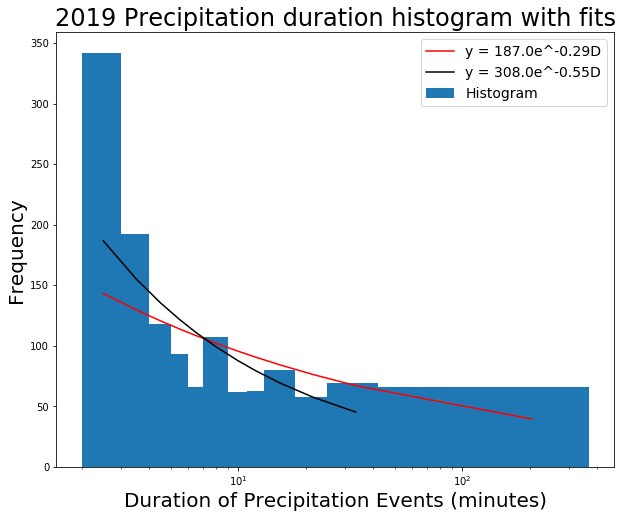
\includegraphics[width=0.675\textwidth]{Figures/precip19_new.png}
\caption[2019 precipitation duration exponentials with contrasting curve
  fitting] {\label{precip19_redone}Curve fitting of the precipitation
  histogram excluding 1 minute duration events for the entire 2019 data. The
  layout is the same as seen in Figure~\ref{precip17_redone}, with 2019
  having complete data like 2018. 2018 and 2019 have similar trends and
  similar curves for both best fit curves.}
\end{figure}

\begin{figure}[b]
\centering
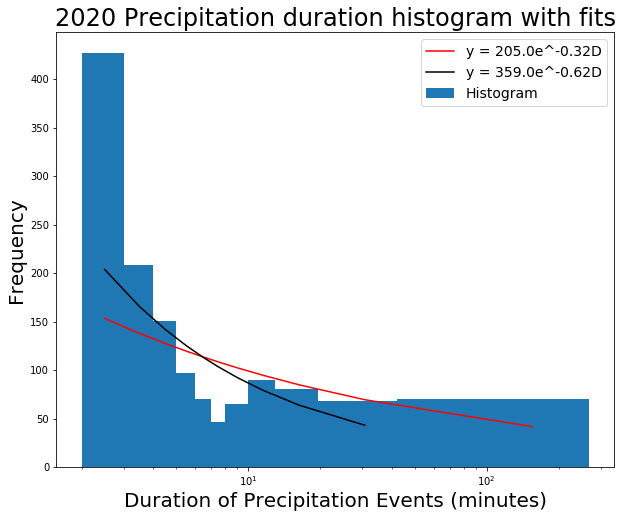
\includegraphics[width=0.675\textwidth]{Figures/precip20_new.png}
\caption[2020 precipitation duration exponentials with contrasting curve
  fitting] {\label{precip20_redone}Curve fitting of the histogram excluding
  1 minute duration events for the entire 2020 data. The layout is the same
  as seen in Figure~\ref{precip17_redone} with 2020 having completed data as
  well. 2018, 2019, and 2020 all look similar looking at the histogram and
  the best fit curves.}
\end{figure}

\clearpage
\begin{figure}[t]
\centering
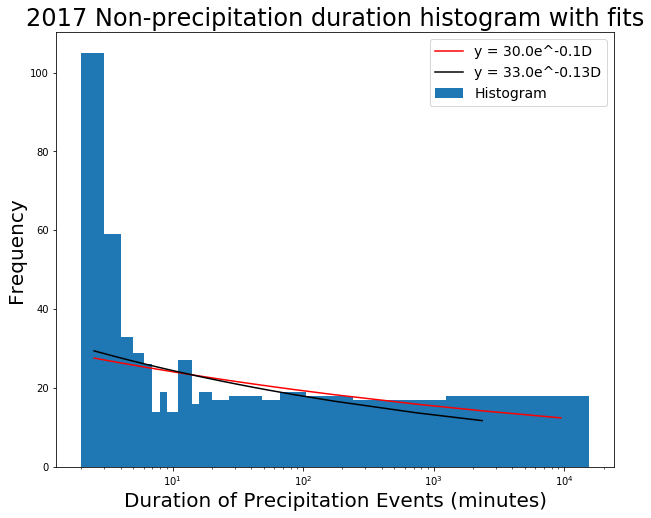
\includegraphics[width=0.625\textwidth]{Figures/nonprecip_2017_new.png}
\caption[2017 Non-precipitation duration Exponentials with contrasting curve
  fitting] {\label{nonprecip17_redone}Curve fitting of the histogram
  excluding 1 minute duration events for the incomplete 2017 data. The red
  curve denotes the curve that fits to the 100th percentile, while the black
  curve fits the data to the 98th percentile. Has similar trends to the
  other years, though 2017 has incomplete data.}
\end{figure}

\begin{figure}[b]
  \centering
  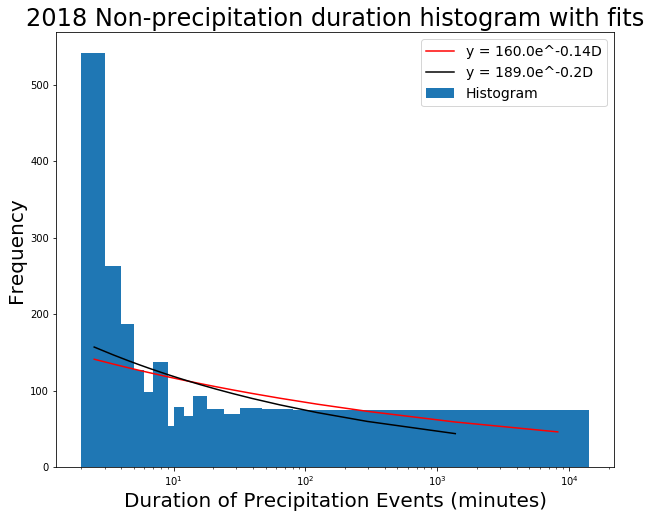
\includegraphics[width=0.625\textwidth]{Figures/nonprecip_2018_new.png}
  \caption[2018 Non-precipitation duration Exponentials with contrasting curve fitting]
  {\label{nonprecip18_redone} Shows curve fitting of the histogram excluding
    1 minute duration events for the entire 2018 data. The red curve denotes
    the curve that fits to the 100th percentile, while the black curve fits
    the data to the 98th percentile. The 98 percentile curve fitting the
    smaller durations better, while the 100 percentile curve fitting the
    larger durations better.  Perhaps the only real difference between 2017
    and 2018 is the frequency, with 2018 having complete data.}
\end{figure}

\clearpage

\begin{figure}[t]
  \centering
  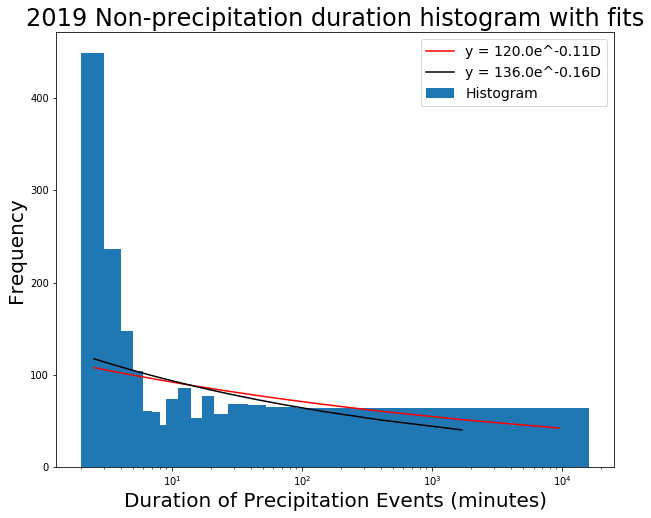
\includegraphics[width=0.675\textwidth]{Figures/nonprecip_2019_new.png}
  \caption[2019 Non-precipitation duration Exponentials with contrasting curve fitting]
  {\label{nonprecip19_redone} Shows curve fitting of the histogram excluding
    1 minute duration events for the entire 2019 data. The layout is the
    same as seen in Figure~\ref{precip18_redone}. 2018 and 2019 have similar trends
    and similar curves for both best fit curves.}
\end{figure}

\begin{figure}[b]
  \centering
  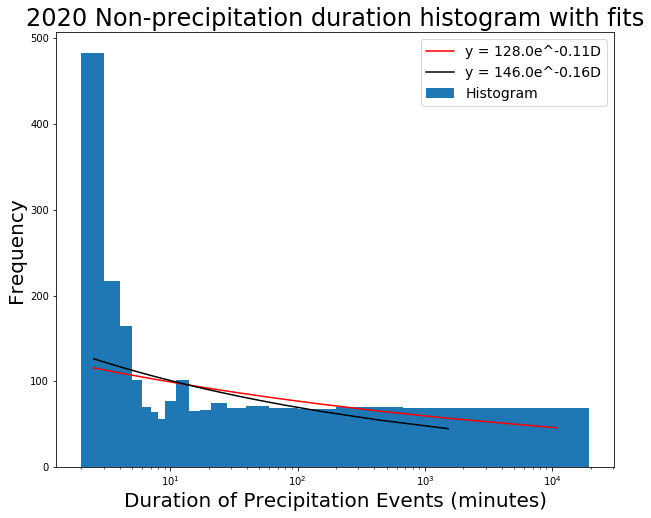
\includegraphics[width=0.675\textwidth]{Figures/nonprecip_2020_new.png}
  \caption[2020 Non-precipitation duration Exponentials with contrasting
    curve fitting] {\label{nonprecip20_redone}Curve fitting of the histogram
    excluding 1 minute duration events for the entire 2020 data. The layout
    is the same as seen in Figure~\ref{nonprecip18_redone}. 2018, 2019, and
    2020 all look similar looking at the histogram and the best fit curves.}
\end{figure}

%Is the exponential different for W/S/S/F? Can you tell the difference?
%Is the exponential different for different years? Can you tell the
%difference?  And what summarizes it all. 
\clearpage
\begin{figure}[t]
  \centering
  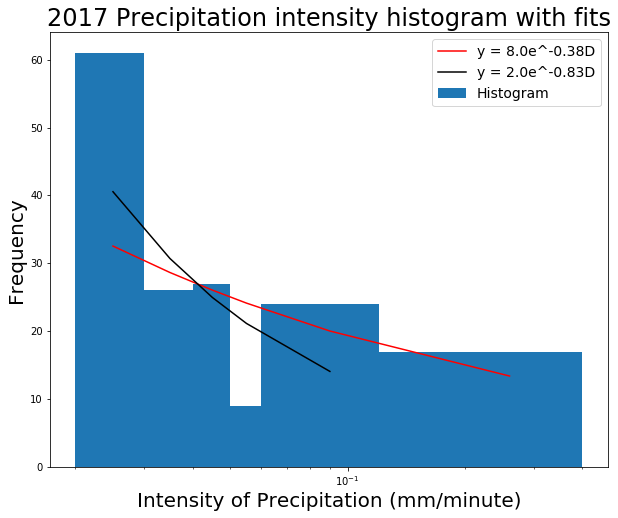
\includegraphics[width=0.675\textwidth]{Figures/inten2017_fit.png}
  \caption[Fitting Intensity histogram for 2017 with different bins]
          {\label{i2017_fit}Curve fitting of the histogram excluding the
            1~mm/minute intensity bin for the 2017 data that was
            collected. The black curve fits up to the 98th percentile
            bin. The red curve fits up to the 100th percentile bin. The
            black curve fits the lower bins better, but the red curve fits
            to include the extremes better.  }
\end{figure}

\begin{figure}[b]
  \centering
  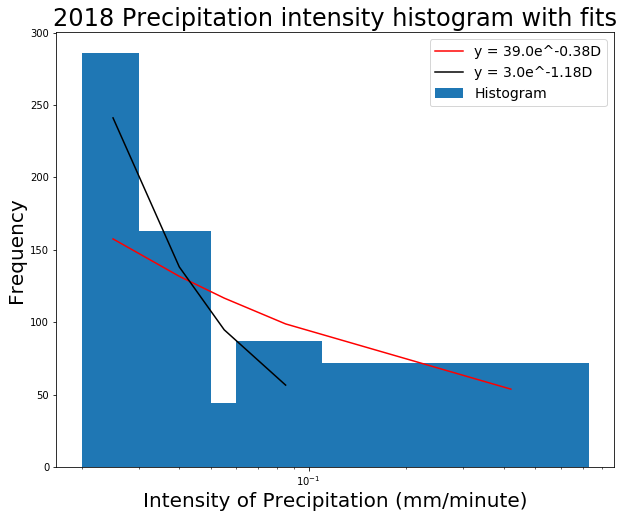
\includegraphics[width=0.675\textwidth]{Figures/inten2018_fit.png}
  \caption[Fitting Intensity histogram for 2018 with different bins]
          {\label{i2018_fit}Curve fitting of the histogram excluding the 1
            mm/minute intensity bin for the entire 2018 data. The layout is
            the same as Figure~\ref{i2017_fit}, with the red curve fitting
            the extremes better, while the black curve fits the lower
            intensity bins better.}
\end{figure}

\clearpage
\begin{figure}[t]
  \centering
  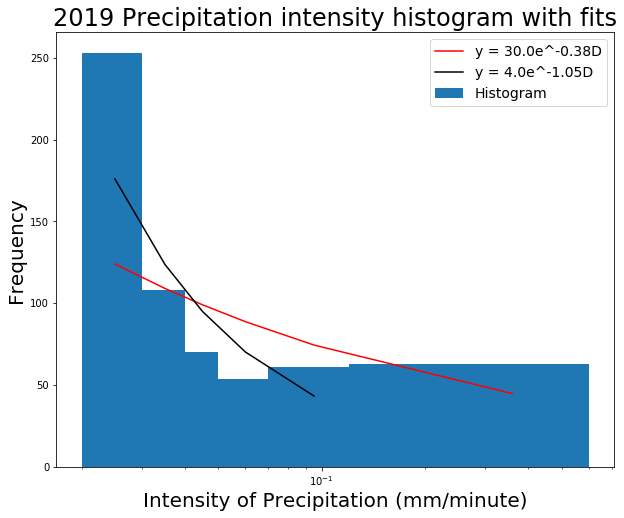
\includegraphics[width=0.675\textwidth]{Figures/inten2019_fit.png}
  \caption[Fitting Intensity histogram for 2019 with different bins]
          {\label{i2019_fit}Curve fitting of the histogram excluding the 1
            mm/minute intensity bin for the entire 2019 data. The layout is
            the same as Figure~\ref{i2017_fit}, with the red curve fitting
            the extremes better, while the black curve fits the lower
            intensity bins better.  }
\end{figure}

\begin{figure}[b]
  \centering
  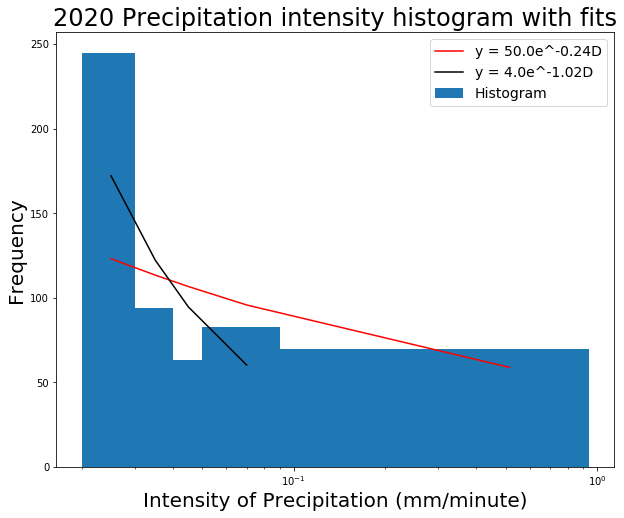
\includegraphics[width=0.675\textwidth]{Figures/inten2020_fit.png}
  \caption[Fitting Intensity histogram for 2020 with different bins]
          {\label{i2020_fit}Curve fitting of the histogram excluding the 1
            mm/minute intensity bin for the entire 2020 data. The layout is
            the same as Figure~\ref{i2017_fit}, with the red curve fitting
            the extremes better, while the black curve fits the lower
            intensity bins better.  }
\end{figure}

\clearpage

\subsection{Discussion}\label{sec:apcd}

Table~\ref{firsttable} show that $\beta$ values are similar to each other
with the exception of 2017, which only had partial data starting in the
summer. Even with the partial data that I have from 2017 and 2020, it is
clear that the $\alpha$ values are similar to each other. Focusing on the
years with complete data, 2018 and 2019, it is clear that yearly variations
exist between them. All $\alpha$ values are negative.\\[-1.5em]

\begin{table}[bh]
  \begin{center}
    \begin{tabular}{|l|*{11}{r|}r|}
      \hline
      Season    &       \multicolumn{2}{|c|}{Annual}          & \multicolumn{2}{|c|}{Winter}& \multicolumn{2}{|c|}{Spring}  & \multicolumn{2}{|c|}{Summer} &\multicolumn{2}{|c|}{Fall}  \\
      \hline
      Year      & $\beta $ & $\alpha$  & $\beta $ & $\alpha$ & $\beta $ & $\alpha$ & $\beta $ & $\alpha$ & $\beta $ & $\alpha$\\
      \hline
      2017      & \textit{169}  & \textit{-0.61}  & NaN & NaN & NaN & NaN & \textit{57}  & \textit{-0.70}  & 108  & -0.57  \\
      2018      & 392           & -0.59  & 148 & -0.74 & 125 & -0.76 & 65  & -0.52  & 91 & -0.50  \\
      2019      & 308           & -0.54  & 118  & -0.62 & 107 & -0.58 & 32 & -0.31  & 57 &  -0.60 \\
      2020      & 408           & -0.65   & 201  & -0.80 & 112  & -0.66 & 48  & -0.42 & 64 & -0.66\\
      \hline
    \end{tabular}
  \end{center}
\caption[Year comparison of coefficients of precipitation duration up to its
  98th percentile]{\label{firsttable}Coefficients found from the yearly
  distribution of precipitation duration (as in equation~\ref{expod}) as
  well as the seasonal distribution of precipitation duration. Italics refer
  to values obtained using incomplete information. NaN means there was no
  information. These coefficients were computed using the 0 to 98th
  percentile of precipitation duration.}
\end{table}


\begin{table}[htb]
  \begin{center}
    \begin{tabular}{|l|*{11}{r|}r|}
      \hline
      Season    &       \multicolumn{2}{|c|}{Annual}          & \multicolumn{2}{|c|}{Winter}& \multicolumn{2}{|c|}{Spring}  & \multicolumn{2}{|c|}{Summer} &\multicolumn{2}{|c|}{Fall}  \\
      \hline
      Year      & $\beta $ & $\alpha$  & $\beta $ & $\alpha$ & $\beta $ & $\alpha$ & $\beta $ & $\alpha$ & $\beta $ & $\alpha$\\
      \hline
      2017      & \textit{94}  & \textit{-0.32}  & NaN & NaN & NaN & NaN & \textit{32}  & \textit{-0.14}  & 68  & -0.09  \\
      2018      & 214           & -0.28  & 73 & -0.37 & 46 & -0.27 & 38  & -0.24  & 55 & -0.23  \\
      2019      & 224          & -0.28  & 68  & -0.34 & 60 & -0.28 & 25 & -0.19  & 33 &  -0.32 \\
      2020      & 234           & -0.35   & 119  & -0.51 & 60  & -0.32 & 36  & -0.27 & \textit{29} & \textit{-0.23}\\
      \hline
    \end{tabular}
  \end{center}
\caption[Yearly comparison of
  coefficients of precipitation duration using 0 to 100th percentile]{\label{firsttable_100} Coefficients found from the yearly
  distribution of precipitation duration (as in equation~\ref{expod})
  as well as the seasonal distribution of precipitation
  duration. Italics refer to values obtained using incomplete
  information. NaN means there was no information. These coefficients were computed using the all the data, from 0 to 100th percentile.}
\end{table}


In the seasonal variations, summer has $\alpha$ values that are
less negative compared to the other seasons as well as having a lower
$\beta$ compared to the other seasons.  The spring appears to mimic the
winter in that there are a lot of preciptiation events, but also shares the
quality of summer in having fairly high precipitation totals. The fall
shares the summer quality of having relatively few preciptation events, but
tends to have smaller precipitation totals, so its intensity is less than
the summer, but greater than the winter precipitation intensity.

Compared to Table~\ref{firsttable}, Table~\ref{firsttable_100} seems to show
$\beta$ values that are consistently lower when considering the 100th
percentile bins for precipitation event durations. The $\alpha$ values are
also less negative, which better reflects that there are extreme durations
for precipitation events.

\ 

\begin{table}[htb]
  \begin{center}
    \begin{tabular}{|l|*{11}{c|}r|}
      \hline Season & \multicolumn{2}{|c|}{Annual} &
      \multicolumn{2}{|c|}{Winter}& \multicolumn{2}{|c|}{Spring} &
      \multicolumn{2}{|c|}{Summer} &\multicolumn{2}{|c|}{Fall} \\ \hline
      Year & $\gamma $ & $\delta$ & $\gamma $ & $\delta$ & $\gamma $ &
      $\delta$ & $\gamma $ & $\delta$ & $\gamma $ & $\delta$\\ \hline 2017 &
      \textit{33} & \textit{-0.13} & NaN & NaN & NaN & NaN & \textit{12} &
      \textit{-0.15} & 19 & -0.12 \\ 2018 & 189 & -0.20 & 59 & -0.28 & 50 &
      -0.29 & 26 & -0.10 & 55 & -0.22 \\ 2019 & 136 & -0.16 & 63 & -0.30 &
      46 & -0.16 & 11 & 0.03 & 24 & -0.16 \\ 2020 & 140 & -0.17 & 64 & -0.23
      & 46 & -0.16 & 13 & -0.02 & 20 & -0.21 \\ \hline
    \end{tabular}
  \end{center}
  \caption[Year comparison of coefficients for non-precipitation events up
    to 98th percentile] {\label{thirdtable_98}Coefficients found from
    the yearly distribution of non-precipitation event duration (as in
    equation~\ref{expod_np}) as well as the seasonal distribution of
    non-precipitation event duration. Italics refer to values obtained using
    incomplete information. NaN means there was no information. Using
    non-precipitation event durations from the 0 to the 98th percentile.}
\end{table}


\begin{table}[htb]
  \begin{center}
    \begin{tabular}{|l|*{11}{c|}r|}
      \hline
      Season    &       \multicolumn{2}{|c|}{Annual}          & \multicolumn{2}{|c|}{Winter}& \multicolumn{2}{|c|}{Spring}  & \multicolumn{2}{|c|}{Summer} &\multicolumn{2}{|c|}{Fall}  \\
      \hline
      Year      & $\gamma $ & $\delta$  & $\gamma $ & $\delta$ & $\gamma $ & $\delta$ & $\gamma $ & $\delta$ & $\gamma $ & $\delta$\\
      \hline
      2017      & \textit{30}  & \textit{-0.10}  & NaN & NaN & NaN & NaN & \textit{11}  & \textit{-0.10}  & 18  & -0.09  \\
      2018      & 160           & -0.14  & 47 & -0.19 & 43 & -0.14 & 23  & -0.05  & 46 & -0.15  \\
      2019      & 120           & -0.11  & 49 & -0.21 & 44 & -0.15 & 11 & 0.04 & 19 & -0.08   \\
      2020      & 121           & -0.11  & 57 & -0.19 & 41 & -0.12 & 12  & 0.01  & 15 & -0.11 \\
      \hline
    \end{tabular}
  \end{center}
  \caption[Year comparison of coefficients for non-precipitation events up
    to 100th percentile] {\label{thirdtable_100}Coefficients found from the
    yearly distribution of non-precipitation event duration (as in
    equation~\ref{expod_np}) as well as the seasonal distribution of
    non-precipitation event duration. Italics refer to values obtained using
    incomplete information. NaN means there was no information. Using
    non-precipitation event durations from the 0 to 100th percentile.}
\end{table}


When fitting non-precipitation event durations using the exponential model,
the coefficients $\delta$ are less negative overall compared to the
coefficients of the precipitation event duration, $\alpha$.

Some of this difference is explained by the fact that the durations of
non-precipitation events range from 1 minute to over 2000 minutes, whereas
the durations of precipitation events range from 1 minute to just over
300--400 minutes. Also, how I bin the durations for both precipitation and
non-precipitation events will affect how the fits are obtained.

Once again, taking into the account the most extreme durations for
non-precipitation events lowers the frequency value of $\gamma$ and the
exponential constant of $\delta$ is less negative, when comparing
Table~\ref{thirdtable_98} and Table~\ref{thirdtable_100}.

\

\begin{table}[htb]
  \begin{center}
    \begin{tabular}{|l|*{11}{c|}r|}
      \hline
      Season    &       \multicolumn{2}{|c|}{Annual}          & \multicolumn{2}{|c|}{Winter}& \multicolumn{2}{|c|}{Spring}  & \multicolumn{2}{|c|}{Summer} &\multicolumn{2}{|c|}{Fall}  \\
      \hline
      Year      & $\epsilon $ & $\zeta$  &  $\epsilon $ & $\zeta$  &  $\epsilon $ & $\zeta$  &  $\epsilon $ & $\zeta$  & $\epsilon $ & $\zeta$ \\
      \hline
      2017      & \textit{0.06}  & \textit{-1.98}  & NaN & NaN & NaN & NaN & \textit{0.03}  & \textit{-1.94}  & 0.04  & -2.00  \\
      2018      & 0.19           & -2.14  & 0.02 & -2.41 & 0.03 & -2.24  & 0.10  & -1.87  & 0.08 & -2.05  \\
      2019      & 0.23           & -2.01  & 0.03 & -2.29 & 0.07 & -2.02 & 0.25 & -1.47 & 0.03 & -2.16  \\
      2020      & 0.06          & -2.38  & 0.002 & -3.00 & 0.02 & -2.38 & 0.10  & -1.74 & 0.02 & -2.18\\
      \hline
    \end{tabular}
  \end{center}
  \caption[Year comparison of coefficients for precipitation
    intensity] {\label{fourthtable}Coefficients found from the yearly
    distribution of precipitation intensity (as in equation~\ref{expod_inten}) as
    well as the seasonal distribution of precipitation
    intensity. Italics refer to values obtained using incomplete
    information. NaN means there was no information. }
\end{table}


\begin{table}[htb]
  \begin{center}
    \begin{tabular}{|l|*{11}{c|}r|}
      \hline
      Season    &       \multicolumn{2}{|c|}{Annual}          & \multicolumn{2}{|c|}{Winter}& \multicolumn{2}{|c|}{Spring}  & \multicolumn{2}{|c|}{Summer} &\multicolumn{2}{|c|}{Fall}  \\
      \hline
      Year      & $\epsilon $ & $\zeta$  &  $\epsilon $ & $\zeta$  &  $\epsilon $ & $\zeta$  &  $\epsilon $ & $\zeta$  & $\epsilon $ & $\zeta$ \\
      \hline
      2017      & \textit{1.6}  & \textit{-1.05}  & NaN & NaN & NaN & NaN & \textit{0.8}  & \textit{-0.94}  & 0.8  & -1.12 \\
      2018      & 12           & -0.919  & 0.7 & -1.36 & 3 & -0.91  & 6  & -0.67  & 4 & -0.91  \\
      2019      & 9           & -0.94  & 0.10 & -1.9 & 3 & -0.94 & 7 & -0.48 & 1 & -1.0  \\
      2020      & 16          & -0.76  & 0.5 & -1.4 & 3 & -0.86 & 13  & -0.32 & 3 & -0.69\\
      \hline
    \end{tabular}
  \end{center}
  \caption[Year comparison of coefficients for precipitation
    intensity using 0 to 100 percentile] {\label{fourthtable_100}Coefficients found from the yearly
    distribution of precipitation intensity (as in equation~\ref{expod_inten}) as
    well as the seasonal distribution of precipitation
    intensity. Italics refer to values obtained using incomplete
    information. NaN means there was no information. Using intensity from 0 to 100th percentile. }
\end{table}


In contrast, Table~\ref{fourthtable} for intensity of precipitation events
show a more negative exponential compared to either precipitation or
non-precipitation event durations. This is partially due to the fact that
there are fewer bins in the intensity of preciptiation events as seen that
the vast majority of precipitation events are not particularly intense on
average.

The differences between Table~\ref{fourthtable} and
Table~\ref{fourthtable_100} show that the exponential coefficients for
intensity clearly are changed most when the 98th percentile or the 100th
percentile are included in the fit. First, the $\epsilon$ value increases
when I use the 100th percentile rather than the 98th
percentile. Furthermore, the $\zeta$ value also becomes less
negative, but very dramatically compared to non-precipitation and
precipitation event durations.

However, Table~\ref{secondtable} shows that the summers also have a lot of
precipitation. There may be fewer precipitation events, but their total
precipitation is higher, hence they have a higher intensity.  For the
winter, the $\alpha$ are the furthest from 0 and the $\beta$ are
large. However, winters tend to have the lowest values for total
precipitation and the combination of lots of preciptation events and low
precipitation totals results in the lowest intensities among the four
seasons.

\begin{table}[t]
  \begin{center}
    \begin{tabular}{|l|*{11}{c|}r|}
      \hline
      Season    &       \multicolumn{2}{|c|}{Annual}          & \multicolumn{2}{|c|}{Winter}& \multicolumn{2}{|c|}{Spring}  & \multicolumn{2}{|c|}{Summer} &\multicolumn{2}{|c|}{Fall}  \\
      \hline
      Year      & T & I  & T & I  & T & I  & T & I  & T & I \\
      \hline
      2017      & \textit{520}  & \textit{0.07}  & NaN & NaN & NaN & NaN & \textit{131}  & \textit{0.07}  & 388  & 0.07  \\
      2018      & 1104           & 0.06  & 147 & 0.03 & 301 & 0.07 & 268  & 0.08  & 388 & 0.07  \\
      2019      & 1016           & 0.06  & 218  & 0.04 & 318 & 0.06 & 352 & 0.11  & 127 &  0.05 \\
      2020      & 858          & 0.06   & 151  & 0.03 & 191  & 0.04 & 322  & 0.12 & 194 & 0.06\\
      \hline
    \end{tabular}
  \end{center}
  \caption[Summary of total precipitation and
    intensity]{\label{secondtable}Total precipitation (in mm) and average
    intensity (in mm/min) of precipitation for each year and season. Italics
    refer to values obtained using incomplete information. NaN means there
    was no information.}
\end{table}

\clearpage

\section{Simulation for Prediction}\label{sec:sfp}

With the exponential distributions calculated from the dataset, I am able
to turn their parameters (precipitation duration, non-precipitation
duration, and intensity) into a climatology-based model to simulate
precipitation and compare such model results to the actual precipitation
data.

\subsection{Method}\label{sec:sfp_m}

To make a baseline model, the exponentials are used to
calculate the duration of the precipitation event, intensity of the
precipitation event, and duration of the non-precipitation events. However,
I also need to manually add back in the lowest durations and lowest
intensities, since I excluded those values when calculating the exponential
distributions. To perform the simulation, I select bins proportionally to
their probability under the distribution, and then pick values from a
uniform distribution with those bins. In order to judge the accuracy of the
model, I count how often model and data agree in the instances where either
model or data have precipiattion present.  This measure of accuracy is
better than simply counting where data and models agree, because
non-precipitation events account for 97\% of the interval under
consideration, in which case the acccuracy would be skewed towards the fact
that most of the time series has no precipitation. 
Another metric that is used is the mean absolute error(MAE), which is measured
when looking time series forecasts. Thus both precipitation accuracy and mean 
absolute error will be calculated for all the following models to come. 

\clearpage
\begin{figure}[t]
  \centering
  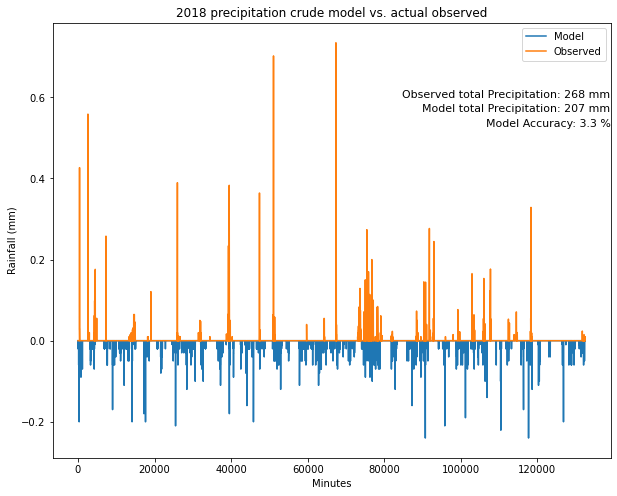
\includegraphics[width=0.65\textwidth]{Figures/better_one_run.png}
  \caption[First run using Summer 2018 climatology] {\label{crudemodel} One
    model run using the 98-percentile exponentials calculated from summer
    2018.}
\end{figure}
\begin{figure}[b]
  \centering
  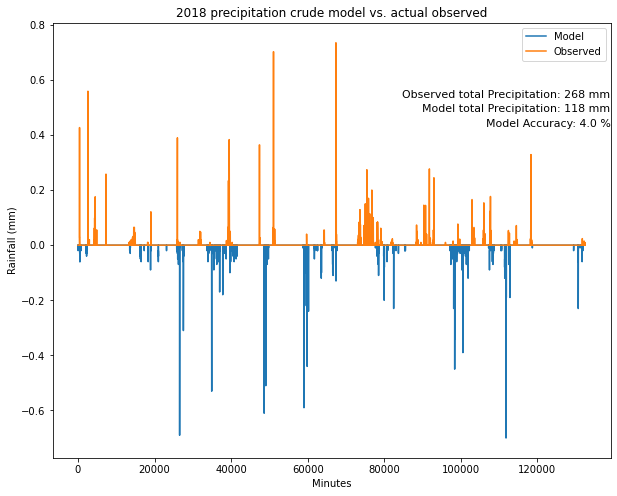
\includegraphics[width=0.65\textwidth]{Figures/best_one_run.png}
  \caption[Modified run using Summer 2018 climatology] {\label{crudermodel}
    A model run using the 100th percentile exponentials calculated from
    summer 2018. The modeled precipitation looks closer to actual
    precipitation. However, the details show they are different: the
    accuracy is only 2.6\% and the total precipitation is still
    underestimated.}
\end{figure}

\clearpage

\subsection{Results}\label{sec:sfp_r}

Running the model one hundred times lets us look at what average total
precipitation the model yields. It yields 215~mm compared to the summer 2018
total of 268~mm in the data that was used for the exponential
fitting. Furthermore, the accuracy of model precipitation matching model
precipitation is only 2.0$\%$ and the MAE is 0.0035~mm/hour. Though running the model 100 times, the model precipitation is 2.5\%. Looking at Figure~\ref{crudemodel}, the model precipitation total is lower than the actual precipitation observed in the summer of 2018. Furthermore, the precipitation seems to be more frequent compared to the observed 2018 summer data. The usage of 98th percentage for all parameters, which are intensity, precipitation event
duration, and non-precipitation event duration, shows that the intensity for
the model is generally good, except the model lacks the most intense values
as expected from the using up to the 98th percentile.

It is clear that despite the better fit that is obtained when the
exponential distributions are fit using data up to the 98th percentile,
the full 100th percentile of the data for the model fitting is useful as well,
since the extremes, such as the big 2000-minute non-precipitation event, are
very important. However, doing that, the precipitation accuracy only goes up 4.0\% and the MAE is 0.0028~mm/hour, as shown in Figure~\ref{crudermodel}. Taking 100 model runs end up giving a precipitation accuracy of 2.6\%. The model total precipitation also gives 118~mm, which is much smaller than the observed precipitation total. 


\subsection{Discussion}\label{sec:spc_d}

Making predictions based on random guesses, however well informed, has
limited success. The accuracy of predicting precipitation, which hovers
around 3\%, shows that no matter how well the three parameters match the
data distributions, simulated time series may not be very accurate.

At the same time, a dilemma arises in which using the 98th percentile
exponentials will return a preciptiation time series that looks nothing like
the observed model, but is close to the value of total precipitation for the
observed model. Using the 100th percentile exponentials will yield a
preciptation time series that looks a lot like the observed precipitation
time series, but will have much less total precipitation compared to the
98th percentile exponential and the observed total precipitation. Despite its flaws, fitting exponentials gives us a good baseline, and it
tells us that there are other methods to look at in order to get a better
model to predict precipitation.

Figure~\ref{crudesmodel_whole2018} is interesting as comparing
the observed 2018 precipitation data to a model run from using the
calculated exponentials for the three parameters I sought to analyze from
the precipitation data. It is clear that the observed data shows that there
are seasonal variations do matter as they have different patterns.  Thus it
validates the notion to split the analysis of the exponentials into the four
seasons, as although its possible to have intense precipitation to occur in
the winter, it is not at all typical of what is usually seen in the winter
and intense precipitation would usually occur in summer.\\[1em]

\begin{figure}[h!]
  \centering
  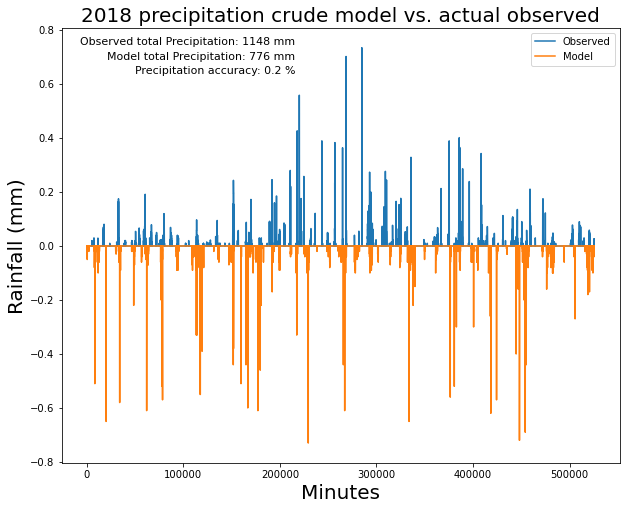
\includegraphics[width=0.75\textwidth]{Figures/whole2018_model.png}
  \caption[Running model for entire 2018 ]
  {\label{crudesmodel_whole2018}One model run using the exponentials calculated from
    the entire year of 2018. }
\end{figure}

\clearpage

\section{Machine Learning for Prediction}\label{sec:MLP}

% FJS Simulation from learned exponential fits gives you a baseline

% FJS ML approach random forest gives you new results

% FJS Contrast with a traditional multiple linear regression

% FJS take into account the time frame for lagged prediction

% Why you need it. 
Although I have one baseline model for predicting precipitation based on
seasonally adjusted historical patterns of precipitation itself, it only
makes point-based instantaneous predictions.  At 2--3\%, its prediction
skill is not very high. Other meteorological variables matter as well, as
will the lead time used for the prediction, and the range of history upon
which it is based.

There are two ways to forecast weather, one is you base forecasting from having lots of emperical data from climatology and weather records. This is the method I had been using up to this point. The other is  dynamics-based forecasts, which involve dynamics equation that govern the atmosphere \cite[]{WF}. Such forecasts use numerical weather prediction (NWP), which involves simulating the atmosphere and its conditions into the future. These models are incredibly complex as they need initial conditions
(often from observations), boundary conditions, and the usage of governing
equations such as physics conservation laws and the ideal gas law. Some
complications of NWP include its inability to simulate small-scale physics
that can affect outcomes, as well as the usage of ensembles, which gives a
variety of predictions based on the small changes in initial conditions
\cite[]{NWP}. 

Now machine learning has arisen as a way to start to evaluate NWPs, such as
predicting at the uncertainity generated by weather forecasts, which 
underperforms NWP uncertainty, it is less computational intensive and beats
other non-NWP methods in calculating uncertainity \cite[]{Scher}.
Machine learning can look at what conditions could yield us precipitation
and how intense it is, which can be less computationally intensive than NWP,
and can give us a good guide on what to expect given certain
conditions.  A method like decision tree can be used to select variables,
assess their relative importance, handle missing values, predict, and
manipulate data. Decision trees are made up of nodes, of which there is the
root node, which represents a choice and a leaf node which represents the
final results of the decision tree. Branches are the choices that are made
from the root nodes \cite[]{DT}.

% Will need a background on so-called "Deep Learning" which is what Neural Networks are part of. 

\subsection{Method}

Two methods from machine learning can be used for predicting
precipitation. Linear regression and decision tree are used to predict
precipitation based on the other parameters that are given to the
model. Linear regression computes the best fit based on the variables you
give and will yield a linear model that relates input data to outcomes.
Decision trees divide the data up into different sections based on certain
criteria. The decision tree can be made to any size, although the size will 
affect how the model divides the data and ultimately the regression. 



\subsection{Results}

Here is a traditional multiple linear regression, training the linear
regression model using 2018 data and trying to predict 2019 precipitation.

The linear regression model is not good at predicting precipitation data. When inputting the 2019 data into the linear regression model, the precipitation that is predicted has a very small intensity. Now, precipitation does tend to see the most precipitation events having a small intensity, however what does not match is the fact that the linear regression model does not have any precipitation events that are more intense than 0.01~mm/minute. The accuracy of predicting precipitation for the model is calculated to be 4.7~\%, which is better than the accuracy from using exponentials to generate random precipitation events. The MAE for the linear regression model is 0.004~mm/hour.


Decision tree is a better predictor of precipitation and how intense the precipitation event is. There are more intense precipitation events as well as less intense precipitation events present when putting in 2019 data to put out a time series for precipitation. The 2019 predicted data have more intense precipitation that occur more often compared to the observed data. There are 6685 minutes of precipitation intensity of 0.1 mm/minute or greater in the 2019 predicted time series. For the observed 2019 precipitation data, there are 2496 minutes of precipitation intensity of 0.1 mm/minute. Also, the 2019 predicted time series ended up having a precipitation total of 2897~mm for the entire year, which is three times higher than the observed 2019 total precipitation. The accuracy of predicting precipitation for decision tree is 11.9\%. The MAE for the decision tree model is 0.007~mm/hour.

\begin{figure}[t]
  \centering
  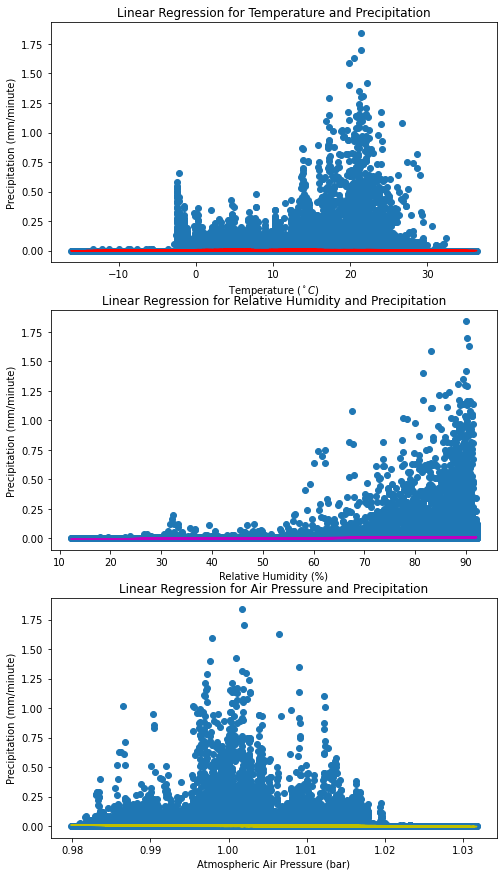
\includegraphics[width=0.75\textwidth]{Figures/ML_Linear_reg.png}
  \caption[ML linear regression run] {\label{ML_Linear}Training the model
    using 2018 data and then using the \textbf{linear regression} model to
    predict 2019 data. Observations are the filled circles, predictions are
    the colored lines. As seen, the linear regression does not do a good job
    in predicting the precipitation, which shows that linear regression is
    not the right method. }
\end{figure}

\begin{figure}[t]
	\centering
	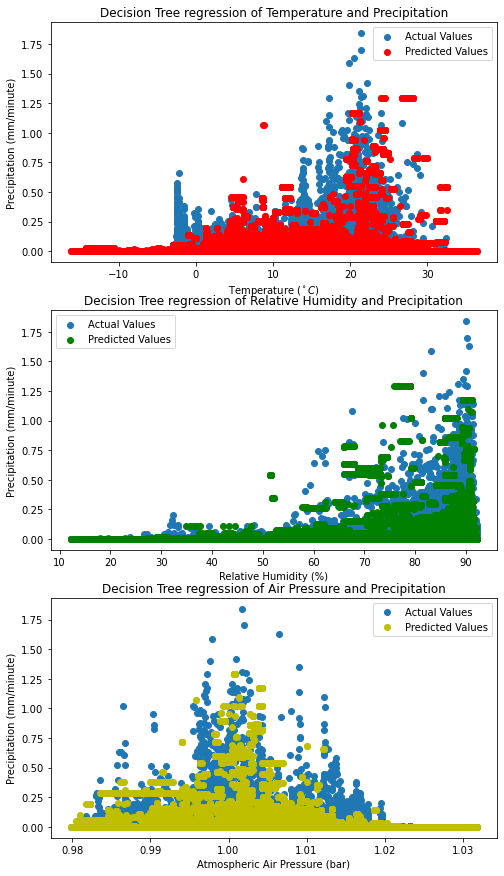
\includegraphics[width=0.7\textwidth]{Figures/ML_DT_reg.png}
	\caption[ML Decision Tree regression run] {\label{ML_DT}Training the
          model using 2018 data and then using the \textbf{decision tree}
          model to predict 2019 data. Decision tree does a better job in
          matching the patterns that are seen with the actual values. At the
          same time, the precipitation accuracy from this one run is 11.9\%}
\end{figure}

\begin{figure}[th!]
  \centering
  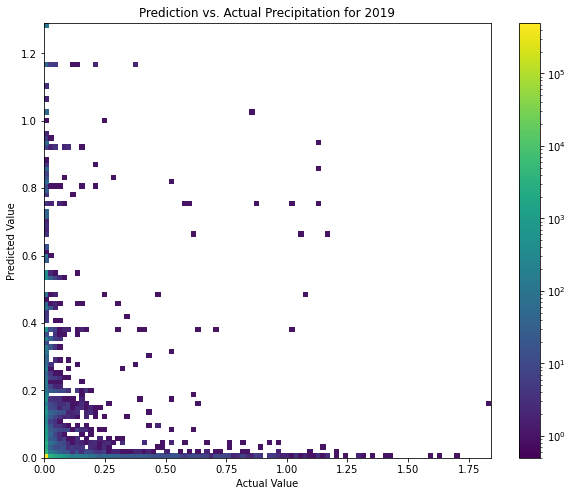
\includegraphics[width=0.7\textwidth]{Figures/predict_and_actual_2019_precip.png}
  \caption[Comparing ML predicted values to actual precipitation
    values]{\label{DT_compare}Comparing the predicted values from decision tree
    regression and the actual values of the 2019 precipitation data.
  }
\end{figure}
\begin{figure}[bh!]
  \centering
  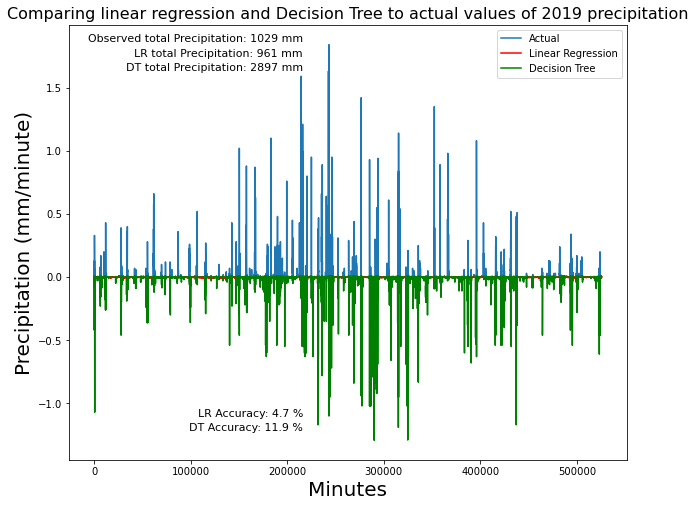
\includegraphics[width = 0.7\textwidth]{Figures/Comparison.png}
  \caption[Comparing ML results to actual precipitation values]{\label{LR_DT_series}
    Comparing the results of linear regression and decision tree
    regression to actual precipitation values of the year 2019. % Note
    %that the total precipitation for observed 2019 is 1029~mm, while
    %the linear regression model, which has negative precipitation, has
    %a total precipitation of 961~mm. Meanwhile the decision tree
    %regression model had a total precipitation of 2941~mm. 
}
\end{figure}

\subsection{Discussion}
It is clear that using linear regression will not do a good job in
predicting precipitation. The low precipitation intensities that come
about is not a problem if not for the fact that there are no intensities
that are larger than 0.01 mm/hour. The extreme precipitation intensities
do exists and can contribute to the total precipitation. In fact, the
linear regression model seems to have events that correspond to negative
precipitation intensity, which is physically impossible. It is a surprise that
the total precipitation does get close to the actual precipitation total of 2019. 

One worry is with decision trees, if you have too many branches, it can
result in overfitting the data, which is not ideal. Our decision tree may
be overfitting, since the total precipitation from the decision tree model gave us 2897~mm, which is 3 times higher than the total observed precipitation of 2019. At first glance, it seems interesting that the linear regression model has a lower precipitation and also a lower MAE compared to the decision tree model. However just looking at how much smaller in magnitude the linear regression model has for the intensity of precipitation and the fact that most of the observed precipitation data is no precipitation at all, so calculating the MAE for linear regression will end up smaller, compared to the decision tree. 

When looking at how many minutes precipitation takes up, the observed 2019 precipitation has 17,000 minutes of precipitation, while the decision tree model has 32,000 minutes of precipitation, and the linear regression model has 362,000 minutes of precipitation. Of course the linear regression model has a maximum precipitation intensity of 0.01~mm/minute. Since the accuracy is calculated from the model precipitation minutes, 3200 minutes from DT matches with the observed precipiation and that 17,000 minutes of precipiation from the linear regression model matches with the observed precipitation data. The linear regression makes a lot of predictions of precipitation when there is not any precipitation, which explains the lower precipitation accuracy, even if it captures all of the observed precipitation. 

\clearpage

\section{Deep Learning for Prediction}\label{sec:neural}

% Why? 
Decision tree and linear regression do lack one thing, in which that time does not matter, so I can put in the data in random order and should get the same results. This should not be a case, in which the data was collected at a specific time. Thus I try using neural networks.

Artificial Neural Networks(ANN) are parallel-distributed information processing system that resembles biological neural network of the human brain \cite[]{ANN}.
With \cite{Norway}, the usage of deep learning on weather data to 
predict temperature hours ahead with good accuracy. However, a variable like temperature is much easier to predict because of the cyclical nature of temperature in both the daily cycle and the annual cycle. LSTM is used because of how it is able to store some memory over an arbitrary amount of time\cite[]{LSTM}. Furthermore, LSTM are good at capturing long-term temporal depedences and the memory cell can maintain its state over time, with gates regulating the flow of information in and out of the cell \cite[]{LSTM_a}. 
  
\subsection{Method}
ANN are made up of three parts. One part is the input layer, which includes a number of input nodes. The second part is one or more hidden layers which include the activation function. The third part is a number of output layer nodes \cite[]{ART}. 


The data is split into at two different datasets, one being the training set and the other being the test dataset. The training dataset is used to fit the model and will consist of one year of the data. When running the model to get the fit based on the training set, the "loss" is calculated by the MAE and a lower MAE is preferred. The test dataset is used to put into the trained model and to evaluate how accurate the model is. To measure how good the model is, precipitation accuracy and MAE are the metrics to use.  


\clearpage

\subsection{Results}

\begin{figure}[th!]
	\centering
	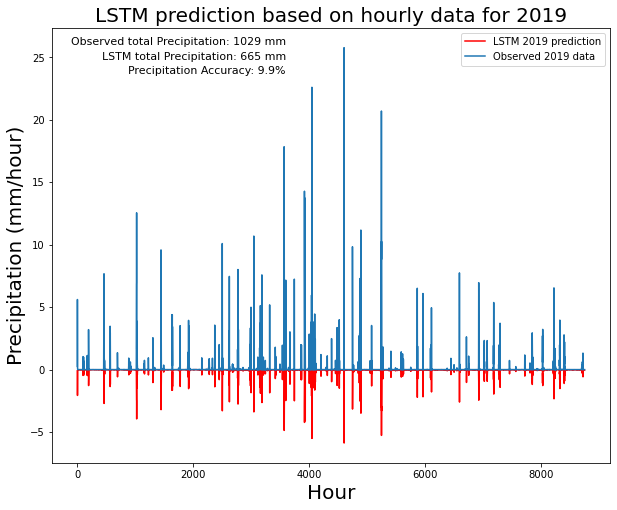
\includegraphics[width = 0.65\textwidth]{Figures/LSTM_hour.png}
	\caption[Comparing LSTM results to observed precipitation in 2019 by hour]{\label{LSTM_hour} Comparing the results of LSTM by hour to the observed
		 precipitation values of the year 2019.
	}
\end{figure}

\begin{figure}[bh!]
	\centering
	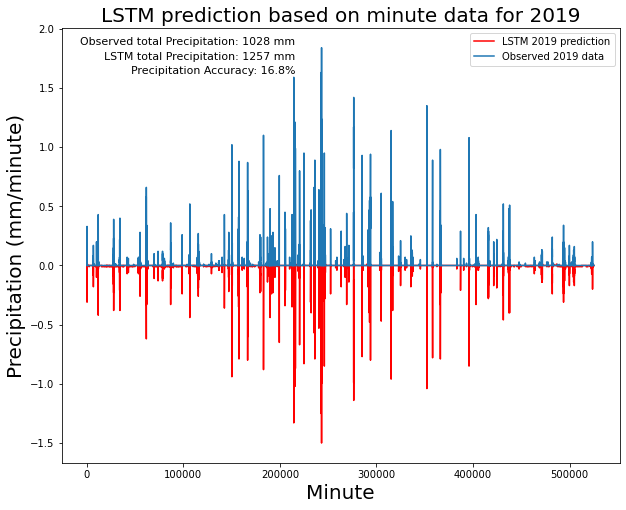
\includegraphics[width = 0.65\textwidth]{Figures/LSTM_minute.png}
	\caption[Comparing LSTM results to observed precipitation in 2019 by minute]{\label{LSTM_minute}
		Comparing the results of LSTM by minute to the observed
		precipitation values of the year 2019.
	}
\end{figure}
\clearpage
\begin{figure}[th!]
	\centering
	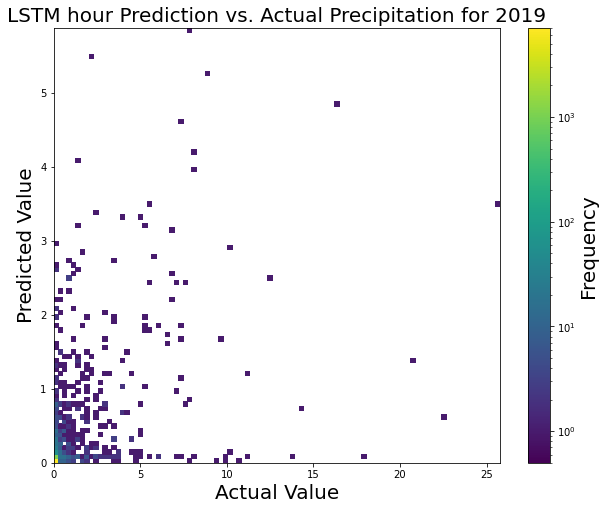
\includegraphics[width = 0.65\textwidth]{Figures/LSTM_hour_compare.png}
	\caption[\label{LSTM_hour_compare}LSTM hour prediction vs. actual data]{
		Comparing the predicted values from LSTM by hour and the actual values of the 2019 precipitation data.
	}
\end{figure}

\begin{figure}[bh!]
	\centering
	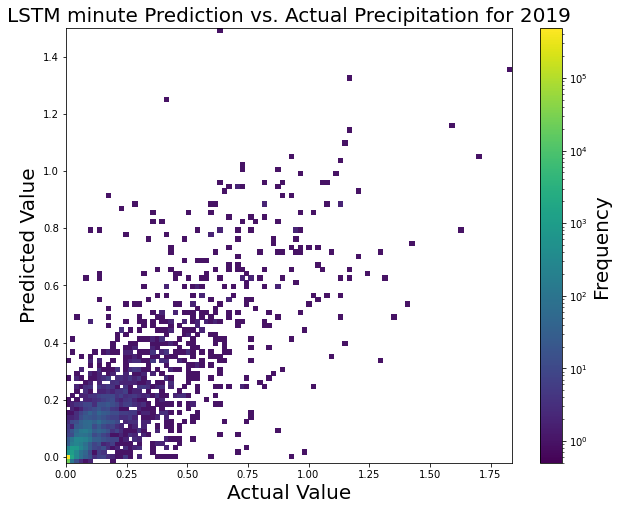
\includegraphics[width = 0.65\textwidth]{Figures/LSTM_minute_compare.png}
	\caption[LSTM minute prediction vs. actual data ]{\label{LSTM_minute_compare}
		Comparing the predicted values from LSTM by minute and the actual values of the 2019 precipitation data.
	}
\end{figure}
\clearpage
For the LSTM by hour model, we end up getting a precipitation accuracy of 9.9\% and an MAE of 0.13~mm/hour. For the LSTM by minute model, we end up getting a precipitation accuracy of 16.8\% and an MAE of 0.0036~mm/minute. Furthermore, we see the behaviors of LSTM better reflect the observed precipitation, with the minute input doing better than the hourly input.  

\subsection{Discussion}
The accuracy of the LSTM model when inputting minute data is higher than the accuracy of the LSTM model when inputting hourly data. However, there are many caveats. In both cases, the predicted precipitation from the LSTM model had more precipitation minutes than actual observed precipitation minutes. Now I figured that many of these cases could be precipitation that lie between 0 mm/minute and 0.01 mm/minute in intensity. Now by rounding the data to the nearest hundredth intensity helped decrease the amount of precipitation minutes that existed in the minute LSTM model. However, there was still a lot more precipitation minutes in the LSTM model than the observed data. This suggests that the LSTM predicts many precipitation events that are not supported by the actual observed data. 

Furthermore, this helps confirm the idea from \cite{CNN} that more frequent inputs improves the accuracy of forecasts. They used the difference between hourly and daily inputs, while I used minute and hourly inputs. Obviously, minute inputs are very numerous and would take a much longer time running such inputs into models in general compared to the hourly inputs. 

The better accuracy is also reflected in the pattern between the predicted LSTM and the observed data. In Figure~\ref{LSTM_minute_compare}, there is a pattern that more closely aligns to a straight diagonal line, which would represent that both the predicted and observed data are of the same precipitation intensity. This is in stark contrast to Figure~\ref{LSTM_hour}, which does not have a good overlap between predicted and observed values and looks closer to Figure~\ref{DT_compare} of poor fits, particularly values that are larger than 0-0.01~mm. 
\clearpage


\section{Discussion and Conclusions}\label{sec:conclusions}


% For the 98 vs. 100th percentile precipitation aspect. 
It is not surprising that looking at two different ranges of data could
affect our analysis. However, it is clear there are benefits and pitfalls
regarding using either percentile. Perhaps the most glaring aspect might
be the handling of extreme precipitation intensity, precipitation event
duration, and non-precipitation event duration. It is clear from the
model based on exponential distribution that the extremes are needed to
get a similar looking time series for precipitation. However, there are
other distributions to consider especially concerning the extremes for
our three parameters. In hydrology,  extreme precipitation intensity uses 
the generalized extreme value (GEV) distribution. This distribution is 
used to confirm the behavior of the tail of rainfall extremes as seen 
in \cite[]{Hydro_dist}, which confirmed previous studies about the 
distribution of extreme rainfall.  

It is also not surprising that using the exponentials to make a model 
that tries to simulate the behavior of the season also does not do too 
well in terms of accuracy. By replicating structure based on the data, 
the model is not trying to match observed precipitation events. 
Thus any matches between the model and the observed data are just 
coincendences. At the same time, it is great that the structures can be
replicated, even if the exact precipitation event can't be predicted. 

Linear regression and decision tree give interesting results, where linear regression can give you a closer total precipitation amount, but decision tree has a larger precipiation accuracy as well as being closer in terms of precipitation minutes that the observed 2019 precipitation data had. Linear regression having a lower MAE compared to the decision tree regression was a surprise at first, but realizing that linear regression being close to 0~mm, meant that its MAE would be calculated to be low, even if it encountered a relatively high precipitation intensity. However, does that mean MAE is not as good of a metric? Hard to say, as the nuances might be with linear regression rather than MAE. 

LSTM usage is interesting because it clearly has the most accurate graph, in which Figure~\ref{LSTM_minute} has the LSTM prediction and the observed data to be very similar to each other, with careful observation to see that the two are not mirror images of each other. At the same time, this similarity is less apparent when looking into how many precipitation minutes were found in LSTM minute, predicted way more minutes than the observed precipitation data. At the same time, LSTM with hourly input having less precipitation accuracy compared to decision tree using minute input was an unexpected find. However, such comparisons are hard to make given different inputs. The precipitation accuracy did improve when going from decision tree with the minute input to LSTM with minute input. 


There is a variety of work that can be done for further work that can done. The first example is using wind as another weather
variable to use to predict precipitation, as one can convert wind
direction and magnitude into 2 components of a wind vector. Another example is
by expanding such analysis to data collected in other stations may be an
interesting path to consider, especially considering that precipitation
can often be predicted based on whether there is precipitation in other
stations/locations as well. 

In terms of future work that can be using neural networks, there are other models to consider. Auto-Regressive Integrated Moving Average(ARIMA) models can be considered as one pathway. For daily weather conditions, ARIMA can be used to forecast meteorological conditions \cite[]{ARIMA}. Future work can implement ARIMA to the weather data to see how it compares to the LSTM model. At the same time, Convoluted Neural Network (CNN) can be used as well. CNNs had been found to have been better than LSTM in prediction of temperature \cite[]{CNN}. There has been a study to suggest that combining CNN and LSTM together may help improve predictions over regular LSTM as well \cite[]{shi2015convolutional}. Interesting to note that ARIMA tends to be used for longer time periods such as monthly or annual, which could mean that such methods can be used for our hourly input or daily inputs. Though it looks like CNN has also been used to make longer time periods predictions like using monthly precipitation \cite[]{Month_CNN}. Now one challenge would be to get more data, which will likely means obtaining data from other weather stations with more extensive records. 

Also looking at the frequency of the most extreme precipitation over a longer period of time may show us climate changing happening in Princeton, as increasing frequency of the most intense rainfall rates may point to climate change. But also looking at the precipitation may also further confirm the pattern discussed in \cite{Held}, where wetter gets wetter and drier gets drier. Obviously such analysis would require many years of data, that does not exist from the Guyot Hall weather station. But any trends in such local data can be compared to other locations to see how the nature of precipitation has changed over time \cite[]{AUST}. Other work can be done using the exponential nature of the three parameters as seen in \cite{Tucker} in looking drainage basin in the context of erosion from precipitation. 

The characterization of precipitation into three parameters of precipitation event duration, non-precipitation event duration, and preciptiation intensity with exponential distribution. The difference between using the 98th percentile and 100th percentile is substantial with the 98th percentile fitting the histograms better, but as seen with the exponential model, the 100th percentile does matter. Using the 98th percentile in the exponential model results in the behavior of the predicted series not matching with the observed data, though better matching the total precipitation.
At the same time, the 100th percentile gives a time series that better matches the behavior of the observed data, but lacking in the total precipitation seen in the observed data. 

As expected, the exponential model was the least accurate in terms of predicting precipitation, with 2-3\% precipitation accuracy. Linear regression and decision tree do a better job of predicting precipitation, with linear regression having a 4.7\% precipitation accuracy and decision tree having a 11.9\% precipitation accuracy. However both linear regression and decision tree suffer from predicting too many precipitation minutes, which is a problem since most of a precipitation time series will be full of zeros. Finally I looked at ANN and using LSTM model for hourly and minute inputs. Hourly inputs for LSTM end up having a precipitation accuracy of 9.9\%, while the minute inputs for LSTM have a precipitation accuracy of 16.8\%. Thus the accuracy increases when going from the exponential model to the ML models to ANN. Further work can help improve the accuracy of such forecasts and to understand the factors that improve or degrade such accuracy. 
%--References
\small
\renewcommand{\bibsep}{0em}

\renewcommand{\bibname}{References}
\bibliographystyle{Latex/gji}
\bibliography{refs}

\clearpage

	\section{Appendix} 
	If you were curious as to how I did my analysis, you are able to replicate such analysis by finding my github account zhangt3-e and going to the repository of senior\_thesis. All the code is under the folder "Code" where you can see many Juypter Notebooks present. Now I will describe the following files to tell you what each file does in alphabetical order. 
	
	Climatology.ipynb takes in all the completed data and summarizes them with climatology. For example, we summarize all the different months using average temperature, monthly precipitation, relative humidity, and air pressure. There is also the summary of the ranges of temperature, relative humidity, and air pressure, as averages can often mask the variations that are present in weather. 
	
	ConvertData.ipynb uses 2018 and 2019 as an example and puts all the data into one text file. It will be useful for those who are not familiar with ASCII files. 
	
	Data\_extract\_and\_histogram.iypnb can be ignored, it was just trying to understand how to deal with the ASCII files that are collected from the weather station. 
	
	Downloadfiles.ipynb is extremely useful if you want to download the ASCII files from Professor Frederik Simon's website. If you want these files for your own local use, this python notebook is extremely useful. 
	
	exponentials.ipynb is the first file to start the actually analysis of the data. This particular file starts the analysis of precipitation event duration and exponential distribution is assumed and thus calculated for both the 98th percentile and the 100th percentile. 
	
	Hist\_func.iypnb was an early attempt to make histograms, but ran into problems of some bins having no frequency, making it harder to do an analysis of histograms. I learned to then use percentiles to make sure I have non-empty bins.
	
	histplot.ipynb contains many essential functions that will be necessary. When trying to use functions from any juypter notebook, you need the import\_ipynb library to be able to import this particular file and to be able to use the function stored here. 
	
	intensity\_and\_non\_precip.ipynb is the file to replicate the analysis of exponentials.ipynb for precipitation intensity and nonprecipitation event durations. 
	
	LSTM.ipynb is the file where I made LSTM analysis on the precipitation data and to predict precipitation data from the trained model. 
	
	ML.ipynb is the file to make predictions using linear regression and decision tree regression on the precipitation data. 
	
	Moredetails.ipynb was the first instance of being able to do a histogram breakdown by seasons as well analysis of the histogram using exponential distribution. 
	
	Neural Networks.ipynb is one attempt at neural networks, although I did not use the results here for my paper. 
	
	season.ipynb is a notebook that analyzed the precipitation data by breaking it down by seasons. It is the blueprint for any analysis of season for any aspect of precipitation. 
	
	Simulation.ipynb is the notebook that contains how to generate a random time series for precipitation based on the exponential distributions of precipitation intensity, precipitation event duration, and non-precipitation event duration. 
	
	Windrose.ipynb was not used in the analysis. However windrose graphs are used to denote direction and magnitude of wind. Of course to be of use, it would be best to convert wind direction and magnitude into vectors that have components of north and east. This can be the starting off of looking at wind as another weather parameter to consider. 
	
	\begin{figure}[h]
		\centering
		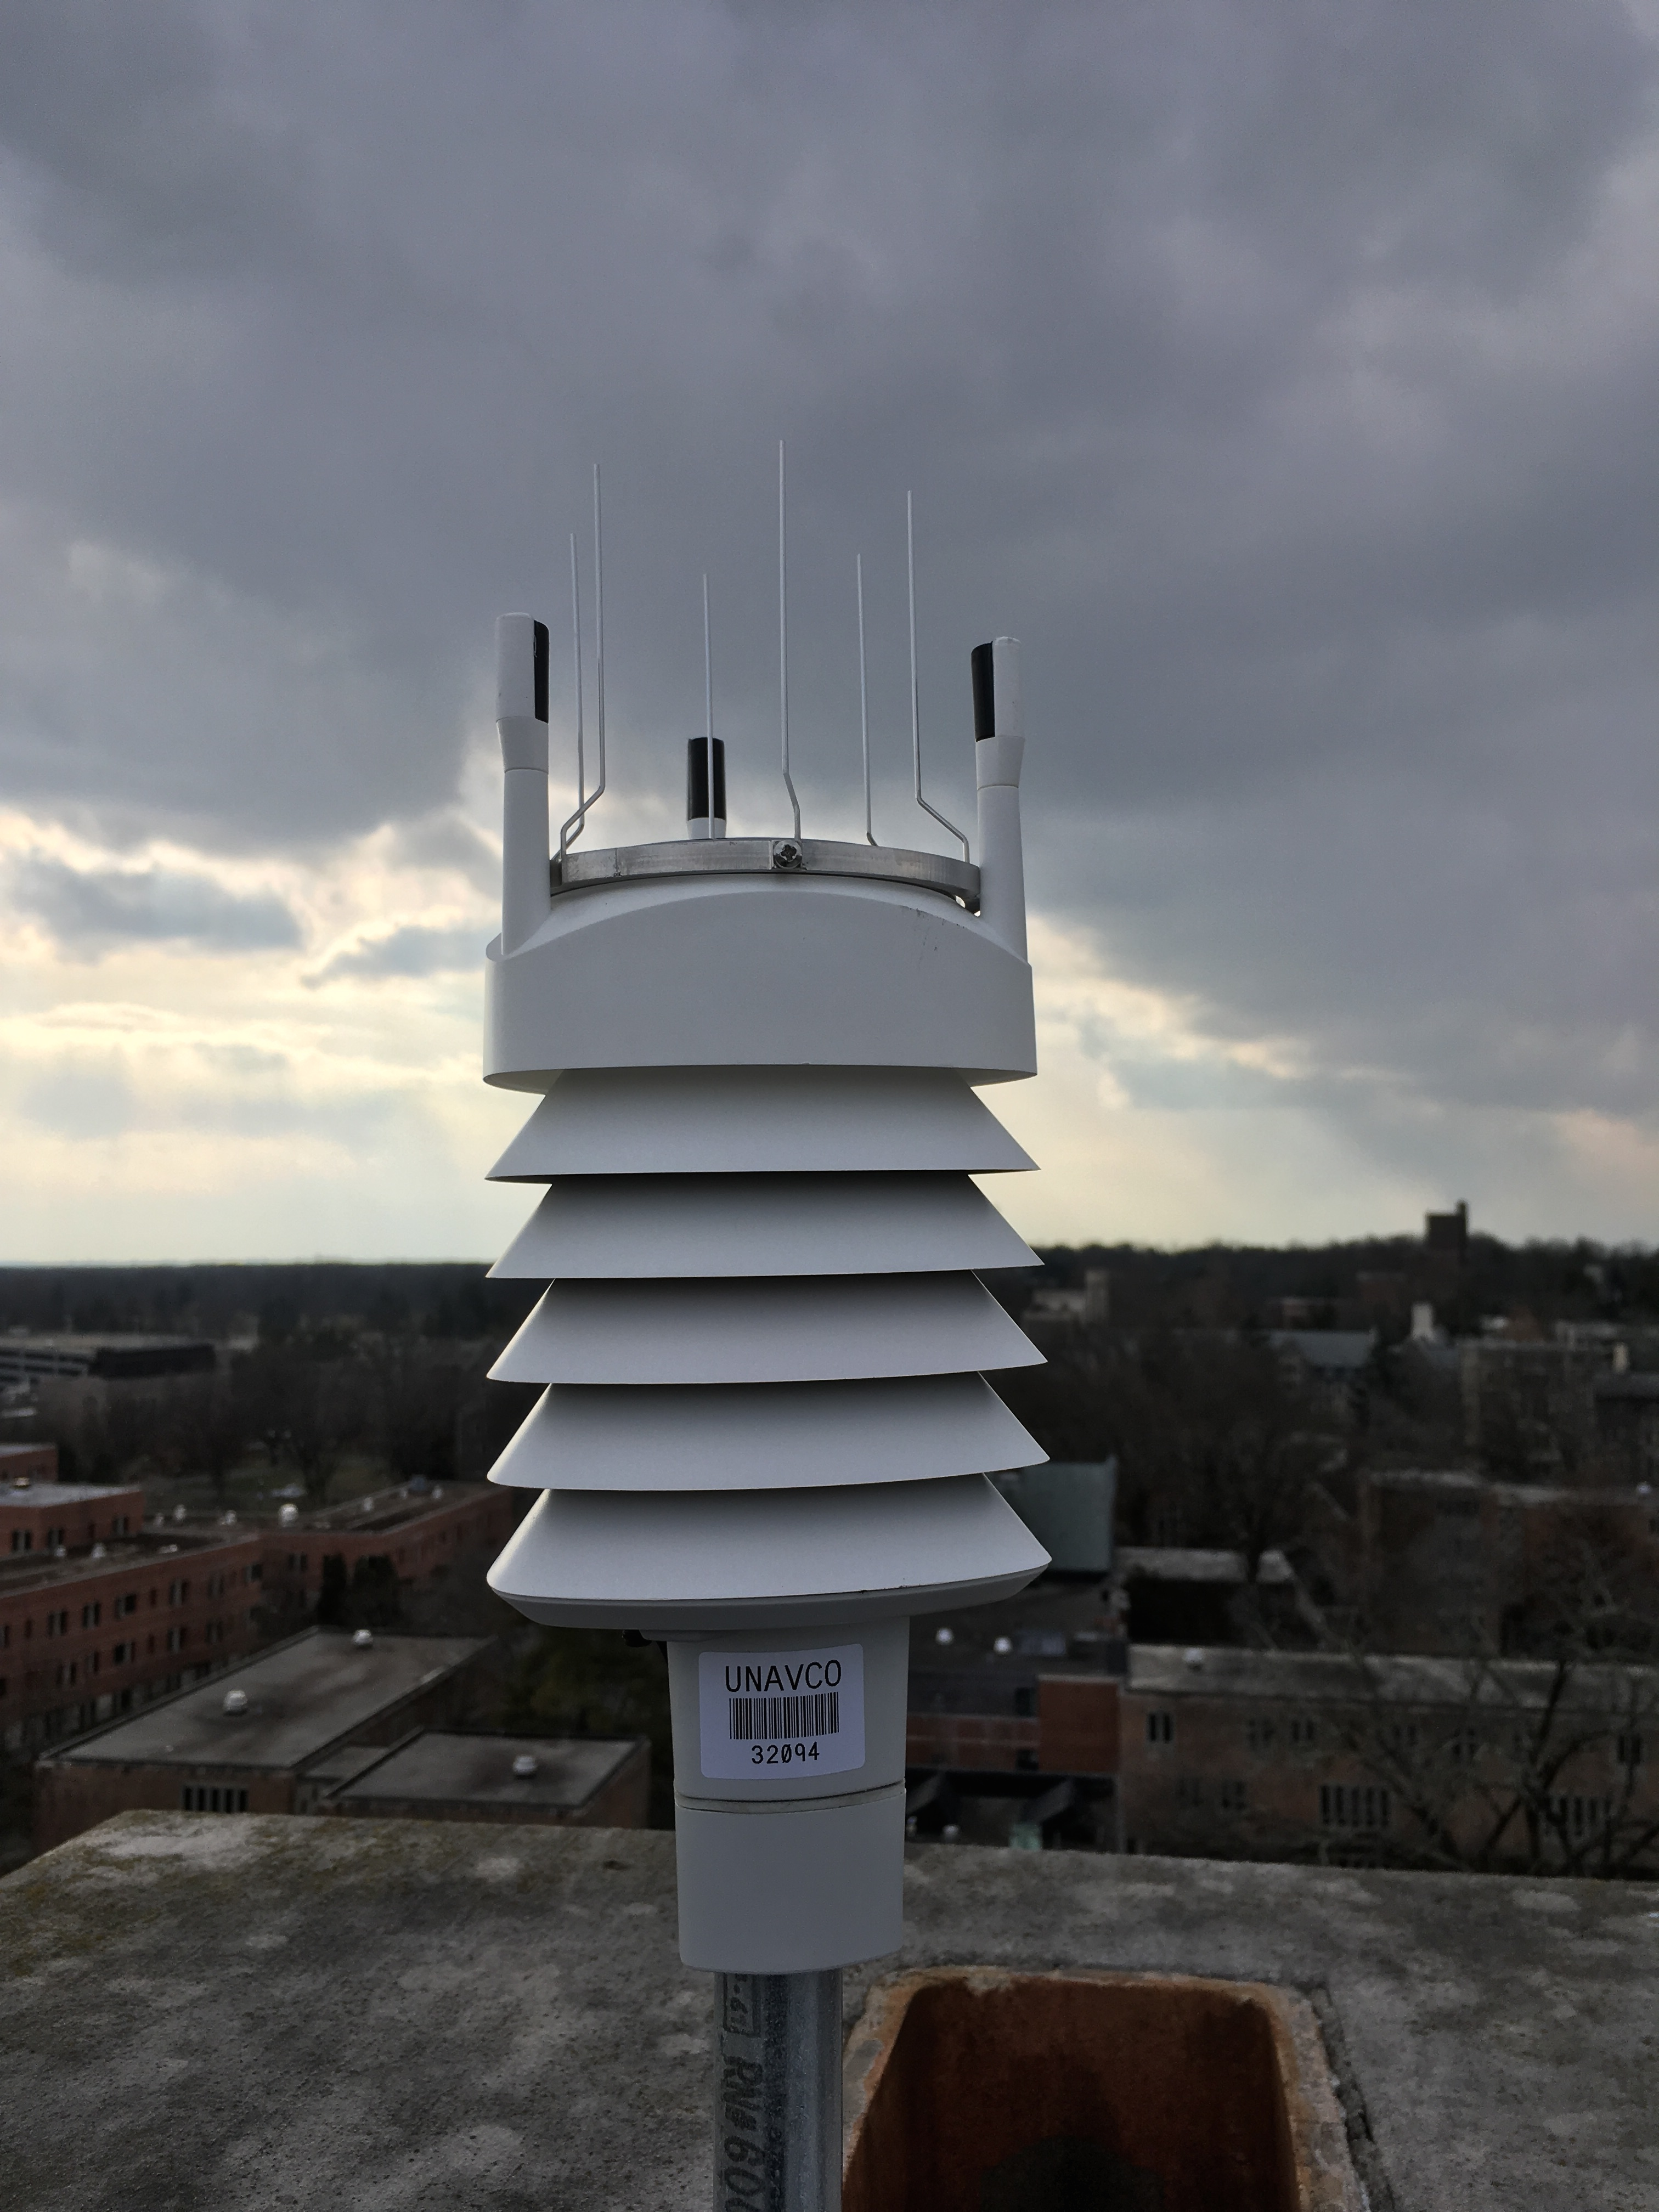
\includegraphics[width = 0.7\textwidth]{Figures/weather_station.jpg}
		\caption[Vaisala Weather Station]{
			Here is the Vaisala Weather Station on top of Guyot Hall.  
		}
	\end{figure}
	
\end{document}

